\documentclass[iop,apj,numberedappendix,twocolappendix]{emulateapj}

\usepackage{mathptmx} % Times for text and math, but sometimes ugly math
                      % (particularly mathcal..)
% \usepackage{times}  % Times but only for text
% \usepackage{apjfonts} % Old workaround that should be similar to mathptmx,
                        % however, clashes with bm
\usepackage[utf8]{inputenc}
\usepackage{amsmath}
\usepackage{amsfonts}
\usepackage{amssymb}
\usepackage{booktabs}
\usepackage{natbib}
\usepackage{graphicx}
\usepackage{aas_macros}
\usepackage[usenames,dvipsnames]{color}
\usepackage{xspace}
\usepackage{bm}
\usepackage{nicefrac}
\usepackage{cancel}
\usepackage{tabularx}
\usepackage{upgreek}	% Url

% \usepackage{fixltx2e} %to display {Figure*}'s in right order

%------------------------------------------------------------------
%\usepackage[notcite,color]{showkeys}%prints all labels in colour or gray, convenient in drafts;
%					%remove "notcite" to show bibliography labels too.
\definecolor{refkey}{rgb}{1,1,1}	%white (invisible) reference keys; use (0,0,1) for blue
\definecolor{labelkey}{rgb}{1,0,0}	%red labels keys
%---------------------------------------------------------------------

\usepackage[normalem]{ulem} %%required for various underlining styles
\usepackage{enumitem} % control of the list indentation & vertical spacing
                      % between the items
\setlist{listparindent=\parindent,leftmargin=*}% indented paragraphs within
                                               % lists,
\usepackage{svn-multi}

%%%%%%%%%%%%%%%%%%%%%%%%%%%%%%%%%%%%%%%%%%%%%%%%
\definecolor{midblue}{rgb}{0.0,0.4,0.7}
\definecolor{midgreen}{rgb}{0.0,0.8,0.3}
\definecolor{mypurple}{rgb}{0.8,0.2,0.8}
\newcommand{\fg}[1]{\textcolor{midblue}{#1}}
\newcommand{\fag}[1]{\textcolor{midgreen}{FAG: #1}}

\def\an{{AN}}
\def\rmp{{Rev.\ Mod.\ Phys.}}
\def\sci{{Science}}

\newcommand{\mathbfss}[1]{\textbf{\textsf{#1}}}
\newcommand\ESK{E_{\rm kin}}
\newcommand\EST{E_{\rm th}}
\newcommand\ESN{E_{\sigma}}
\newcommand\Ms{M_{\rm s}}
\newcommand\Rm{{\rm Rm} }
\newcommand\Rey{{\rm Re} }
\newcommand\Pm{{\rm Pm} }
\newcommand\kf{k_{\rm f} }
\newcommand\BKM{{\sf BKMM4}}
%
%       UNITS
%
  \newcommand{\cm}{\,{\rm cm}}
  \newcommand{\mm}{\,{\rm mm}}
  \newcommand{\dyn}{\,{\rm dyn}}
  \newcommand{\erg}{\,{\rm erg}}
  \newcommand{\g}{\,{\rm g}}
  \newcommand{\Jy}{\,{\rm Jy}}
  \newcommand{\Jyb}{\,{\rm Jy/beam}}
  \newcommand{\km}{\,{\rm km}}
  \newcommand{\kms}{\,{\rm km\,s^{-1}}}
  \newcommand{\mJy}{\,{\rm mJy}}
  \newcommand{\mJyb}{\,{\rm mJy/beam}}
  \newcommand{\K}{\,{\rm K}}
  \newcommand{\kpc}{\,{\rm kpc}}
  \newcommand{\p}{\,{\rm pc}}
  \newcommand{\Mpc}{\,{\rm Mpc}}
  \newcommand{\Myr}{\,{\rm Myr}}
  \newcommand{\Gyr}{\,{\rm Gyr}}
  \newcommand{\mG}{\,{\rm mG}}
  \newcommand{\mkG}{\,\mu{\rm G}}
  \newcommand{\nG}{\,{\rm nG}}
  \newcommand{\MHz}{\, {\rm MHz}}
  \newcommand{\Msol}{\,{\rm M_{\sun}}}
  \newcommand{\radm}{\,{\rm rad\,m^{-2}}}
  \newcommand{\s}{\,{\rm s}}
  \newcommand{\yr}{\,{\rm yr}}

  \newcommand{\lo}{l_{0}}
  \newcommand{\vect}[1]{\boldsymbol{#1}}
  \newcommand{\dd}{\mathrm{d}}
  \newcommand{\dx}{\delta x}
  \newcommand\SNr{\dot\sigma_{\rm sn}}

  % MNRAS conventions for software names
  \newcommand{\pencil}{\textsc{pencil}\xspace}

% for the ``ArXivish'' bib version ----------------------------------
\usepackage[breaklinks,colorlinks,
  urlcolor=blue,citecolor=blue,linkcolor=blue,pdfborder={0 0 0.1}]{hyperref}
% Metadata for the PDF file (will be useful in a very distant future...)
\hypersetup{
pdftitle={Large- and small-scale dynamo modes the supernova driven turbulence},
pdfauthor={
            F.~A.~Gent (orcid.org/0000-0002-1331-2260),
            M-M.~{Mac Low}, (orcid.org/0000-0003-0064-4060)
            M.~J.~K\"apyl\"a (orcid.org/0000-0002-9614-2200),
            N.~Singh, % (orcid.org/?)
          }
}

% Choose favorite figures for arXiver website https://arxiver.wordpress.com/
%@arxiver{alpha1beta1.pdf,beta_dep_uu.pdf,RM_structure_functions.pdf}

\shorttitle{Large- and small-scale dynamo modes the supernova driven turbulence}
\shortauthors{F.~A.~Gent, M-M.~{Mac Low}, M.~J.~K\"apyl\"a, N.~Singh}

% \received{2014 Month DD}
% \accepted{2014 Month DD}
% \published{2014 Month DD}
% \journalinfo{The Astrophysical Journal, ddd:dd (ddpp), 2014 Month DD}

\begin{document}

\begin{abstract}
tba
\end{abstract}

\title{Large- and small-scale dynamo modes the supernova driven turbulence}
\author{F.~A.~Gent,\altaffilmark{1}
  M-M.~{Mac Low},\altaffilmark{2} M.~J.~K\"apyl\"a,\altaffilmark{1,3} 
  and N.~Singh\altaffilmark{3}
}

\affil{
$\sp{1}$ ReSoLVE Centre of Excellence, Department of Computer Science, Aalto University, PO Box 15400, FI-00076 Aalto, Finland \\
$\sp{2}$ American Museum of Natural History, 79th Street at Central Park West, New York, NY 10024, USA\\
$\sp{3}$ Max Planck Institute for Solar System Research, Justus-von-Liebig-Weg 3, 37707 G\"ottingen, Germany
}

\email{
       frederick.gent@aalto.fi (FAG)
       }

\keywords{galaxies: ISM -- ISM: kinematics and dynamics -- ISM: magnetic fields -- turbulence -- methods: statistical
}

%-------------------------------------------------------------------------
\section{Introduction}
\label{sect:introduction}
tba 

%-------------------------------------------------------------------------------------------------
\section[]{Shock tests}
\label{sect:shocks}

%-------------------------------------------------------------------------
\begin{figure*}
\centering
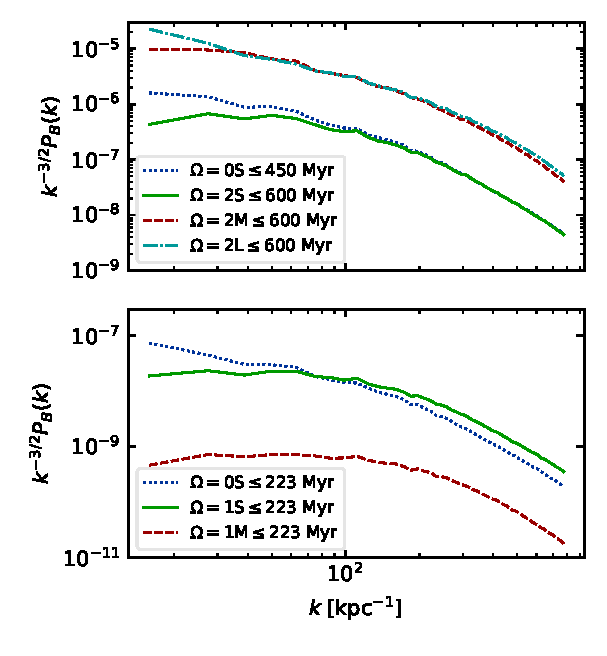
\includegraphics[trim=0.0cm 0.0cm 0.0cm 0.0cm,clip=true,width=0.49\textwidth]{csc_figs/B1O1qMBpower.pdf}
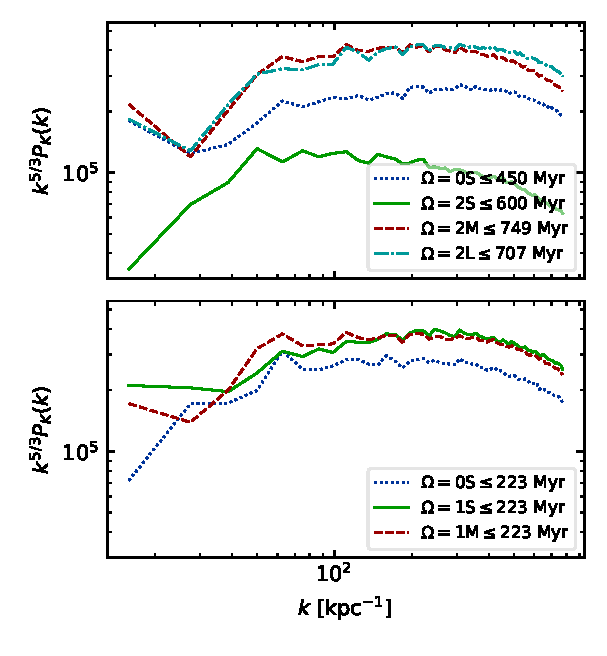
\includegraphics[trim=0.0cm 0.0cm 0.0cm 0.0cm,clip=true,width=0.49\textwidth]{csc_figs/B1O1qMkpower.pdf}
\caption{
Compensated power spectra at $\dx=4$\,pc averaged over 5\,Myr preceding time
and for rotation rate $\Omega$ as indicated in the legends, and with 
shear ratio $q=1.5$ (upper) and 1 (lower) for magnetic energy (left) and
kinetic energy (right).
Legend labels S, M and L indicate azimuthal length $Ly=0.512,\,1.024$ and 
1.536\,kpc, respectively. 
\label{fig:lsd-power}
}
\end{figure*}
%--------------------------------------------------------------------------

%-------------------------------------------------------------------------
\begin{figure}
\centering
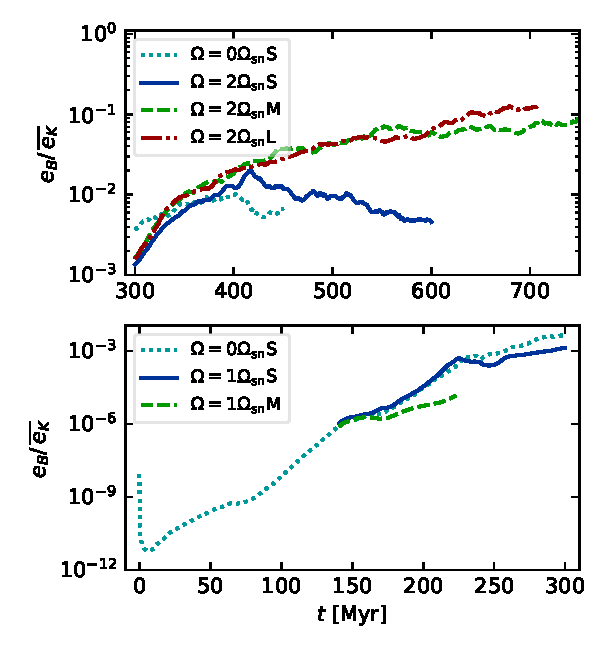
\includegraphics[trim=0.0cm 0.0cm 0.0cm 0.0cm,clip=true,width=0.45\textwidth]{csc_figs/eB-res-4eta.pdf}
\caption{
Magnetic energy density, $e_B$, normalised by time averaged kinetic energy 
density, $\overline{e_K}$, at $\dx=4$\,pc with rotation rate $\Omega$ as
indicated in the legends, and shear ratio $q=1.5$ (upper) and 1 (lower). 
Legend labels S, M and L indicate azimuthal length $Ly=0.512,\,1.024$ and 
1.536\,kpc, respectively. 
\label{fig:lsd-eB}
}
\end{figure}
%--------------------------------------------------------------------------

%-------------------------------------------------------------------------
\begin{figure}
\centering
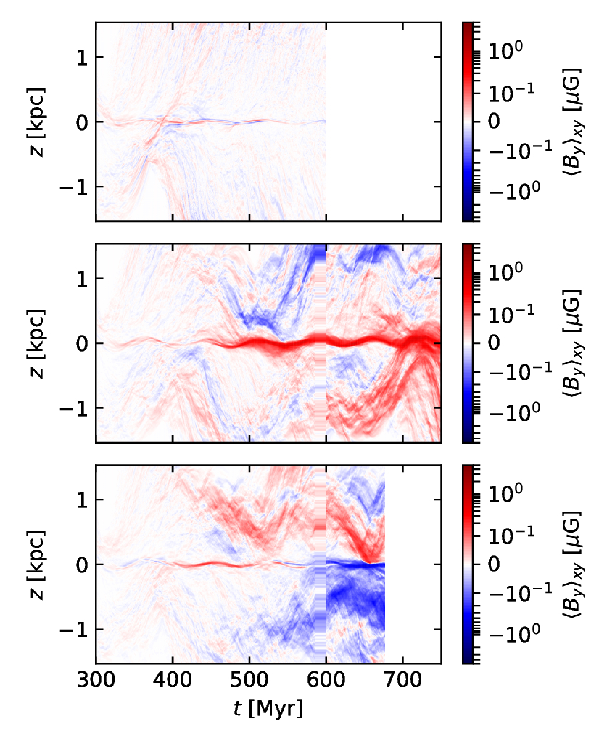
\includegraphics[trim=0.0cm 0.0cm 0.0cm 0.0cm,clip=true,width=0.5\textwidth]{csc_figs/av-bymzsm.pdf}
\caption{
Horizontally averaged azimuthal magnetic field, $B_y$, at $\dx=4$\,pc for 
stratified ISM with rotation rate $\Omega=2\Omega_{\rm sn}$ and shear ratio
$q=1.5$.
The azimuthal extent of the domain $L_y=0.512$\,kpc (upper), 1.024 (centre) 
and 1.536 (lower). 
\label{fig:lsd-bymz}
}
\end{figure}
%--------------------------------------------------------------------------

%-------------------------------------------------------------------------
\begin{figure}
\centering
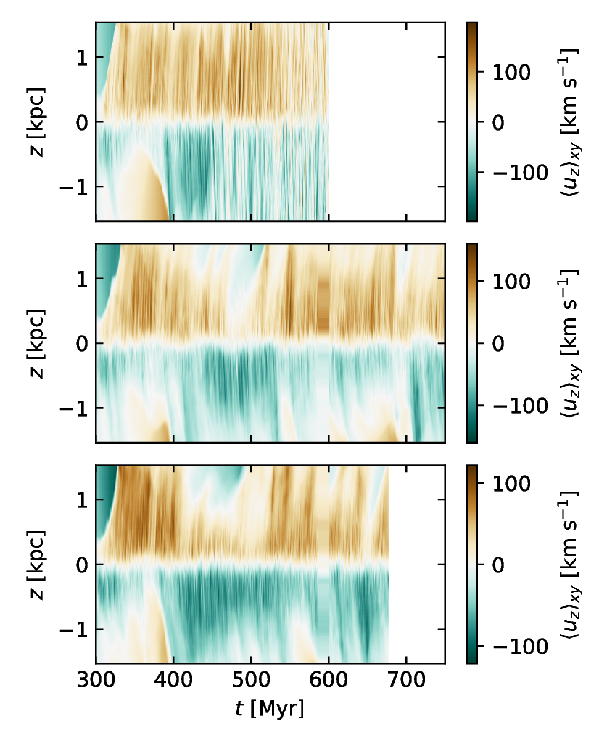
\includegraphics[trim=0.0cm 0.0cm 0.0cm 0.0cm,clip=true,width=0.5\textwidth]{csc_figs/av-uzmzsm.pdf}
\caption{
Horizontally averaged vertical velocity, $u_z$, at $\dx=4$\,pc for 
stratified ISM with rotation rate $\Omega=2\Omega_{\rm sn}$ and shear ratio
$q=1.5$.
The azimuthal extent of the domain $L_y=0.512$\,kpc (upper), 1.024 (centre) 
and 1.536 (lower). 
\label{fig:lsd-uzmz}
}
\end{figure}
%--------------------------------------------------------------------------

%-------------------------------------------------------------------------
\begin{figure}
\centering
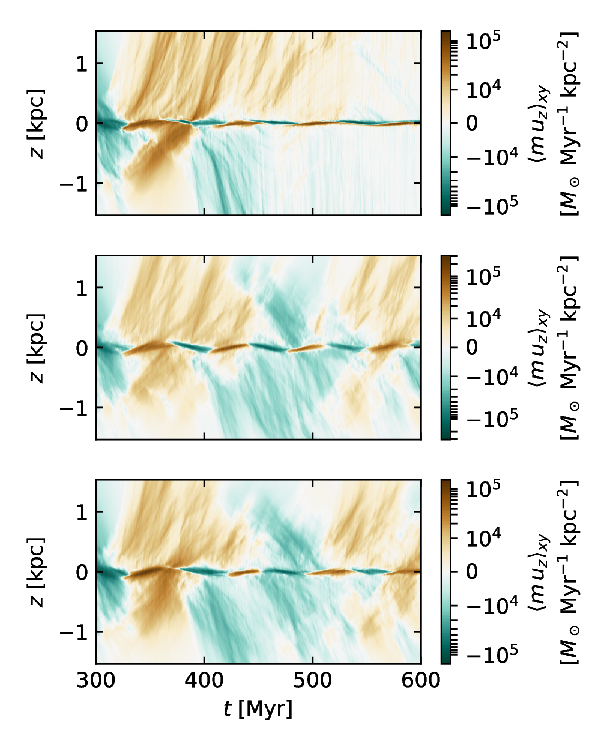
\includegraphics[trim=0.0cm 0.0cm 0.0cm 0.0cm,clip=true,width=0.5\textwidth]{csc_figs/av-ruzmzsm.pdf}
\caption{
Horizontally averaged vertical momentum, $m\,u_z$, at $\dx=4$\,pc for 
stratified ISM with rotation rate $\Omega=2\Omega_{\rm sn}$ and shear ratio
$q=1.5$.
The azimuthal extent of the domain $L_y=0.512$\,kpc (upper), 1.024 (centre) 
and 1.536 (lower). 
\label{fig:lsd-ruzmz}
}
\end{figure}
%--------------------------------------------------------------------------

%-------------------------------------------------------------------------
\begin{figure}
\centering
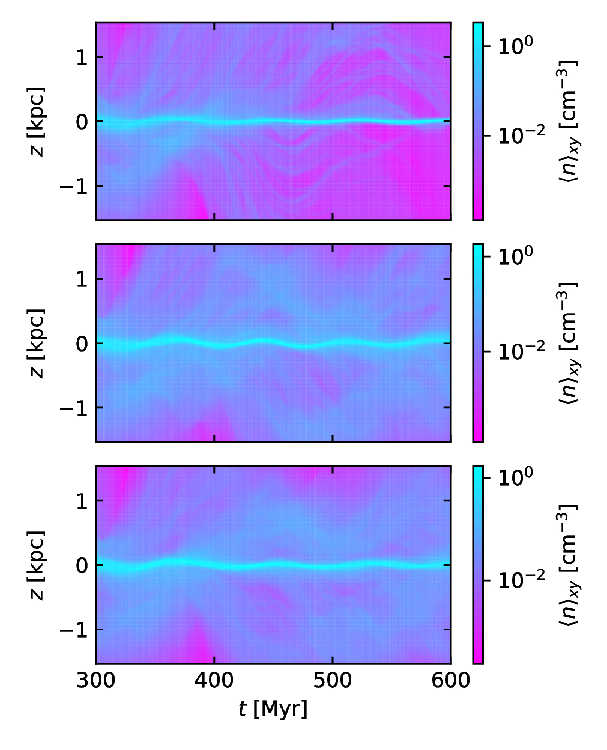
\includegraphics[trim=0.0cm 0.0cm 0.0cm 0.0cm,clip=true,width=0.5\textwidth]{csc_figs/av-rhomzsm.pdf}
\caption{
Horizontally averaged gas number density, $n$, at $\dx=4$\,pc for 
stratified ISM with rotation rate $\Omega=2\Omega_{\rm sn}$ and shear ratio
$q=1.5$.
The azimuthal extent of the domain $L_y=0.512$\,kpc (upper), 1.024 (centre) 
and 1.536 (lower). 
\label{fig:lsd-rhomz}
}
\end{figure}
%--------------------------------------------------------------------------

%-------------------------------------------------------------------------
\begin{figure}
\centering
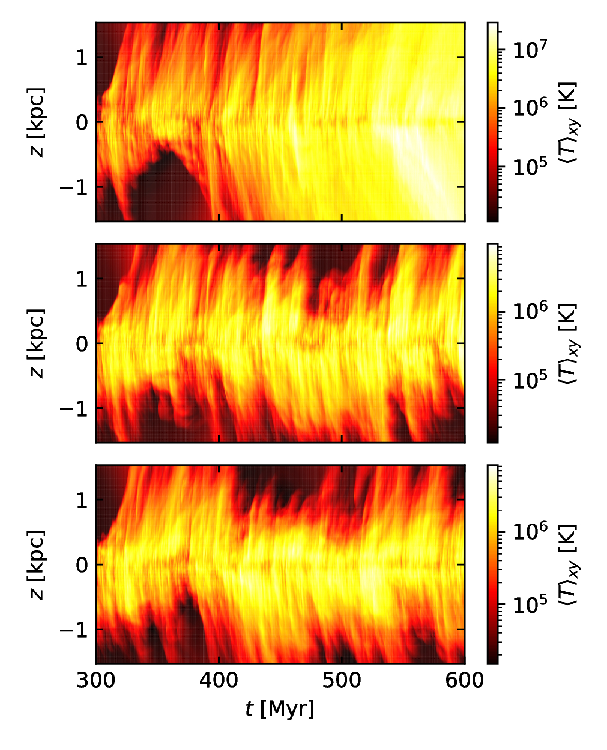
\includegraphics[trim=0.0cm 0.0cm 0.0cm 0.0cm,clip=true,width=0.5\textwidth]{csc_figs/av-ttmzsm.pdf}
\caption{
Horizontally averaged gas temperature, $T$, at $\dx=4$\,pc for 
stratified ISM with rotation rate $\Omega=2\Omega_{\rm sn}$ and shear ratio
$q=1.5$.
The azimuthal extent of the domain $L_y=0.512$\,kpc (upper), 1.024 (centre) 
and 1.536 (lower). 
\label{fig:lsd-ttmz}
}
\end{figure}
%--------------------------------------------------------------------------

%In all Figures\,\ref{fig:weakshock}--\ref{fig:adiabvcooling} a shock diffusion 
%proportional to a quadratic dependence on the convergence of the flow is
%applied for viscosity, $\nu$, and thermal diffusivity, $\chi$. 
%The shock viscosity follows \citet{SN92} and a similar prescription is
%implemented for the divergence of the temperature gradient in the energy 
%equation.
%Hence, enhanced diffusion is applied proportional to  
%$|(\mathbf{\nabla}\cdot\mathbf{u})_{-}|^2$ only where convergence
%is non-zero.
%Hyperdiffusion is applied in the form of upwind everywhere.
%The coefficients applied are $\nu_{\rm shock}, \chi_{\rm shock}=2.0$ 
%\footnote{Fred: Note $\nu_{\rm shock}\mathbf{\nabla}\cdot\mathbf{u}$ has the same dimension as the Laplacian viscosity $\nu\sim[L]^2[t]^{-1}$, but in the energy
%equation $\chi_{\rm shock}(\mathbf{\nabla}\cdot\mathbf{u})^2$ has dimension
%$\sim[L]^2[t]^{-2}$.
%This requires a substantially larger coefficient, of order a few hundred,
%for it to become dynamically effective.
%For now I have included a further division by $\Delta x$, so that applying the
%same value 2.0 with the current grid resolution
%(effective $\chi_{\rm shock}/\Delta x=800$) seems to be effective.
%However, the scaling should have dimension $[t]$ rather than $[L]^{-1}$, to
%ensure it remains constant as resolution varies.
%Any ideas?
%}
\section[]{Models}
\label{sect:models}
 We solve the system of non-ideal compressible MHD equations
%-------------------------------------------------------------------------------
  \begin{eqnarray}
  \label{eq:mass}
    \frac{D\rho}{Dt} &=& \fg{\rho_{\rm sn}\dot\sigma}
    -\rho \vect\nabla \cdot \vect{u}
    +\vect\nabla \cdot\zeta_D\vect\nabla\rho,
  \end{eqnarray}
%-------------------------------------------------------------------------------
  \begin{eqnarray}
  \label{eq:mom}
    \rho\frac{D\vect{u}}{Dt} &=& 
    \vect\nabla{\ESK\sigma}
    -\rho c_{\rm s}^2\vect\nabla\left({s}/{c_{\rm p}}+\ln\rho\right)
    +\vect{j}\times\vect{B} + \fg{\rho\vect{g}}
    \nonumber\\
    &+&\vect\nabla\cdot \left(2\rho\nu{\mathbfss W}\right)
    +\rho\,\vect\nabla\left(\zeta_{\nu}\vect\nabla \cdot \vect{u} \right)
    \nonumber\\
    &+&\vect\nabla\cdot \left(2\rho\nu_3{\mathbfss W}^{(3)}\right)
  {-\vect u\vect{\nabla}\cdot\left(\zeta_D\vect{\nabla}\rho\right)},
  \end{eqnarray}
%-------------------------------------------------------------------------------
  \begin{eqnarray}
  \label{eq:ent}
    \rho T\frac{D s}{Dt} &=&
     \EST\dot\sigma +\rho\Gamma
    -\rho^2\Lambda +\eta\mu_0\vect{j}^2 
    \nonumber\\
    &+&2 \rho \nu\left|{\mathbfss W}\right|^{2}
    +\rho\,\zeta_{\nu}\left(\vect\nabla \cdot \vect{u} \right)^2
    \nonumber\\
    &+&\vect\nabla\cdot\left(\zeta_\chi\rho T\vect\nabla s\right)
    +\rho T\chi_3\vect\nabla^6 s
    \nonumber\\
    &-& {c_{\rm{v}}\,T \left(
    \zeta_D\nabla^2\rho + \vect\nabla\zeta_D\cdot\vect\nabla\rho\right)},
  \end{eqnarray}
%-------------------------------------------------------------------------------
  \begin{eqnarray}
  \label{eq:ind}
    \frac{\partial \vect{A}}{\partial t} &=&
    \vect{u}\times\vect{B}
    +\eta\vect\nabla^2\vect{A}
    +\eta_3\vect\nabla^6\vect{A},
  \end{eqnarray}
%-------------------------------------------------------------------------------
 with the ideal gas equation of state closing the system.
 Most variables take their usual meanings.
 Terms containing $\zeta_D{=2},\,\zeta_\nu{=5}$ and $\zeta{_\chi=2}$
 {are applied to all ISM models and} resolve shock discontinuities with
 artificial diffusion of mass, momentum, and energy proportional to shock
 strength \citep[see][for details]{GMKSH20}.
 Equations~\eqref{eq:mom} and \eqref{eq:ent} include terms with $\zeta_D$
 {to} {provide momentum and energy conserving corrections for} {the}
 {artificial mass diffusion applying in \eqref{eq:mass}.}
 Shock diffusion is not applied to equation~\eqref{eq:ind}{, unlike} {in}
 {\citet{Gent:2013b}.} {This avoids} {excessive magnetic dissipation in
 shocks, where compression actually enhances it.}
 Terms containing $\nu_3,\,\chi_3$ and $\eta_3$ apply sixth-order hyperdiffusion
 to resolve grid-scale instabilities \citep[see, e.g.,][]{ABGS02,HB04}, {
 with coefficients optimal for each $\dx$}.

 {The simplified isothermal model considered above
 (Sect.\,\ref{sec:ssd-tang}) solves only equations~{\eqref{eq:mass},}
 \eqref{eq:mom} and~\eqref{eq:ind}, without the shock-dependent diffusion or
 hyperdiffusion terms, and while setting
 $\vect{B}=\vect\nabla\times\vect{A}+\vect{B}_{\rm imposed}$.}

 {In the ISM simulations} SNe are exploded at {uniform} random positions
 at a Poisson rate $\dot\sigma$ {scaled by} the solar neighborhood
 value $\SNr\simeq 50\kpc^{-3}\Myr^{-1}$.
 Explosions inject $\EST = 10^{51}\erg$ thermal energy, except in
 dense regions, where a proportion {($<5\%$) may be} kinetic $\ESK$ 
 \citep[see][]{GMKSH20}.
 {Models with common $\dot\sigma$ have the same timing and location of
 explosions.}
 Non-adiabatic heating $\Gamma$ and cooling $\Lambda (T)$ are included
 \citep{Gent:2013b} following \citet{Wolfire:1995} and \citet{Sarazin:1987}.


 {Unlike past} experiments \citep{Gent:2013b,Gent:2013a,GMKSH20},
 thermal diffusivity, $\chi$, {is omitted as} the artificial diffusivities
 are adequate to ensure numerical stability.
 {The} physical effects of thermal conductivity can be expected to be
 relevant only at the unresolved or marginally resolved Field length defined
 by \citet[][named after George Field, not the magnetic field]{BM90}.
 {For comparison to our models with physical diffusivity and understanding
 of the effects of purely numerical diffusivity, we also run an ideal MHD model
 with} $\eta=0$ {and $\nu=0$.}

 We determine how low a physical resistivity $\eta$ can be resolved by varying
 it from $10^{-5}$ to $10^{-3}\kpc\kms$ (units assumed henceforth).
 {We also test the effect of $\Pm=\nu/\eta$, varying $\nu$ with 
 $\eta=10^{-4}$ or varying $\eta$ with $\nu=10^{-3}$.}
 {Our direct comparison with the results of \BKM\ uses $\Pm=2.5$, apart
 from one run using $\eta=\nu=0$.}
 
\section[]{Modelling supernova explosions}
\label{sect:SNe}

Our numerical prescription for applying supernova modelling has been described
in \citet{GSFSM13,Gent2012}.
Revisions have been included to improve numerical stability, improve accuracy 
of the remnant evolution within regions of high density ISM, and preserve gas
in the disk for the duration of the simulations.
We, therefore, take this opportunity to present a comprehensive description of
our treatment of SNe.

We implement Type II SN and Type Ic SN, which differ in our models only by the
rate at which they explode and how their positions are vertically distributed.



%-------------------------------------------------------------------------
\begin{figure*}
\centering
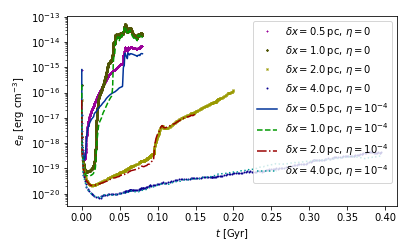
\includegraphics[trim=0.0cm 0.0cm 0.0cm 0.0cm,clip=true,width=0.47\textwidth]{csc_figs/eB-res-4eta.png}
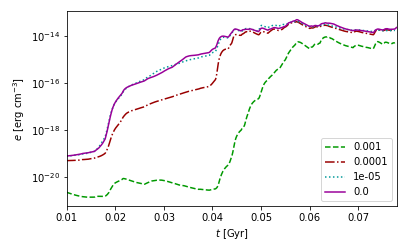
\includegraphics[trim=0.0cm 0.0cm 0.0cm 0.0cm,clip=true,width=0.47\textwidth]{csc_figs/1pc-eB-nu.png}
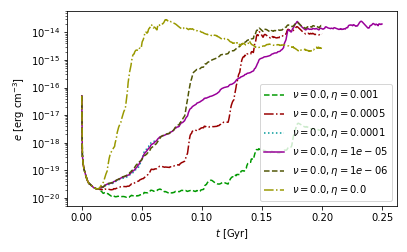
\includegraphics[trim=0.0cm 0.0cm 0.0cm 0.0cm,clip=true,width=0.47\textwidth]{csc_figs/2pc-eB-nu.png}
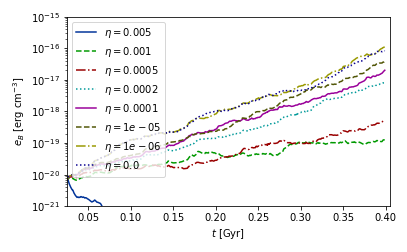
\includegraphics[trim=0.0cm 0.0cm 0.0cm 0.0cm,clip=true,width=0.47\textwidth]{csc_figs/4pc-eB-nu.png}
\caption{
Panel {\bf(a)}: for resolution of 0.5, 1, 2 and 4\,pc the magnetic energy for
models with hyper diffusion coefficients 
${\cal{D}}_{3}=10^{-15.5},\,10^{-14.5},\,10^{-13.1}$ and $10^{-11.7}$,
respectively.
For resolution 1, 2  and 4\,pc, the respective ${\cal{D}}_{3}$ together with 
$\eta\in[0,10^{-2.3}]$ and $\nu=0$, in panels {\bf(b)} to {\bf(d)},
respectively.
${\cal{D}}_{3}=[\nu_3,\chi_3,\eta_3]$ and ${\cal{D}}_1=[\nu,\eta]$.
\label{fig:brms}
}
\end{figure*}
%--------------------------------------------------------------------------

%-------------------------------------------------------------------------
\begin{figure*}
\centering
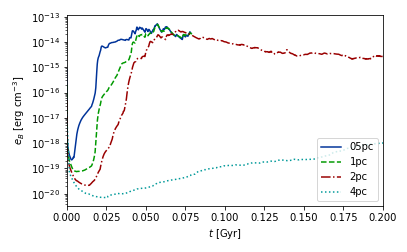
\includegraphics[trim=0.0cm 0.0cm 0.0cm 0.0cm,clip=true,width=0.47\textwidth]{csc_figs/eB-res-zoom.png}
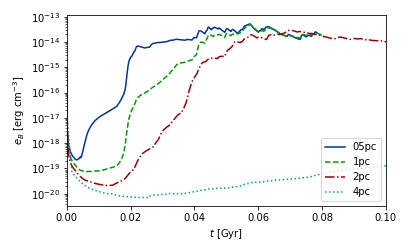
\includegraphics[trim=0.0cm 0.0cm 0.0cm 0.0cm,clip=true,width=0.47\textwidth]{csc_figs/eB-res-2xzoom.png}
\caption{
Zoomed in time intervals of Figure\,\ref{fig:brms} panel\,{\bf(a)} of the magnetic energy growth rates for various spatial resolution.  
\label{fig:brms_res_zoom}
}
\end{figure*}
%--------------------------------------------------------------------------

%-------------------------------------------------------------------------
\begin{figure*}
\centering
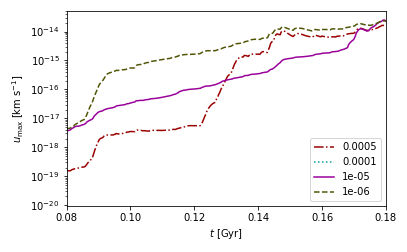
\includegraphics[trim=0.0cm 0.0cm 0.0cm 0.0cm,clip=true,width=0.47\textwidth]{csc_figs/2pc-eB-zoom.png}
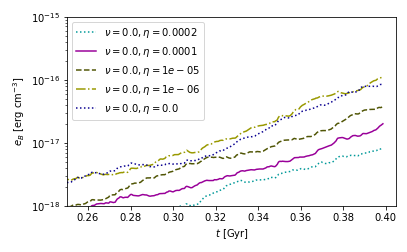
\includegraphics[trim=0.0cm 0.0cm 0.0cm 0.0cm,clip=true,width=0.47\textwidth]{csc_figs/4pc-eB-zoom.png}
\caption{
Zoom in at 2\,pc and 4\,pc resolution of the magnetic energy growth rates with  
${\cal{D}}_{3}=10^{-13.1},\,10^{-11.7}$, respectively, $\eta\in[0,10^{-3.3}]$ and $\nu=0$.
\label{fig:brms_zoom}
}
\end{figure*}
%--------------------------------------------------------------------------

%-------------------------------------------------------------------------
\begin{figure*}
\centering
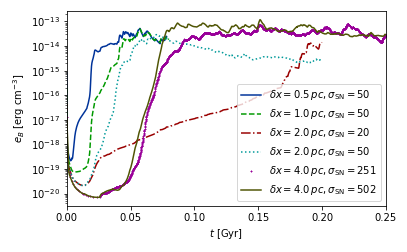
\includegraphics[trim=0.0cm 0.0cm 0.0cm 0.0cm,clip=true,width=0.47\textwidth]{csc_figs/sn_dx.png}
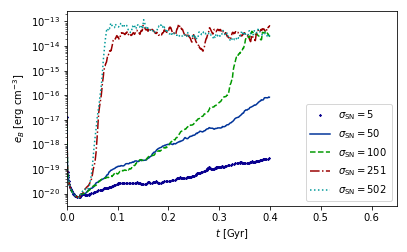
\includegraphics[trim=0.0cm 0.0cm 0.0cm 0.0cm,clip=true,width=0.47\textwidth]{csc_figs/sn4pc.png}
\caption{
Effect of supernova rate, $\sigma_{\rm SN}$ [kpc$^{-3}$Myr$^{-1}$], at various
spatial resolution. Panel (b) 4\,pc with $\sigma_{\rm SN} \in[5,502]$.
{Remember to comment that we compared constant heating vs \citet{Wolfire:1995} et al and this was not significant.}
\label{fig:brms_SNrate}
}
\end{figure*}
%-------------------------------------------------------------------------

%\begin{table*}
%\begin{tabular}{lcccccccc}
%\input{tables/4pc_01SNseedstats}
%\input{tables/4pc_2SNseedstats}
%\input{tables/4pc_5SNseedstats}
%\input{tables/4pc_10SNseedstats}
%\end{tabular}
%\end{table*}
%
%%--------------------------------------------------------------------------
%
%\begin{table*}
%\begin{tabular}{lcccccccc}
%\input{tables/4pc_h5seedstats}
%\input{tables/4pcPm0e-5.0stats}
%\input{tables/4pcPm0e-4.0stats}
%\input{tables/4pcPm0e-3.7stats}
%\input{tables/4pcPm0e-3.3stats}
%\input{tables/4pcPm0e-3.0stats}
%\input{tables/4pcPm0e-2.3stats}
%\end{tabular}
%\end{table*}
%%-------------------------------------------------------------------------
%
%%-------------------------------------------------------------------------
%
%\begin{table*}
%\begin{tabular}{lcccccccc}
%\input{tables/4pcPm0e-0_02SNstats}
%\input{tables/4pcPm0e-4_02SNstats}
%\input{tables/4pcPm0e-3_02SNstats}
%\end{tabular}
%\end{table*}
%
%%--------------------------------------------------------------------------
%
%\begin{table*}
%\begin{tabular}{lcccccccc}
%\input{tables/2pc_h5seedstats}
%\input{tables/2pcPm0e-5.0stats}
%\input{tables/2pcPm0e-5.0stats}
%\input{tables/2pcPm0e-4.0stats}
%\input{tables/2pcPm0e-3.3stats}
%\input{tables/2pcPm0e-3.0stats}
%\end{tabular}
%\end{table*}
%%-------------------------------------------------------------------------
%\begin{table*}
%\begin{tabular}{lcccccccc}
%\input{tables/2pcPm0e-0_02SNstats}
%\input{tables/2pcPm0e-4_02SNstats}
%\input{tables/2pcPm0e-3_02SNstats}
%\end{tabular}
%\end{table*}
%%-------------------------------------------------------------------------
%
%\begin{table*}
%\begin{tabular}{lcccccccc}
%\input{tables/1pcPm0e-0.0stats}
%\input{tables/1pcPm0e-5.0stats}
%\input{tables/1pcPm0e-4.0stats}
%\input{tables/1pcPm0e-3.0stats}
%\end{tabular}
%\end{table*}
%
%%-------------------------------------------------------------------------
%
%\begin{table*}
%\begin{tabular}{lcccccccc}
%\input{tables/0.5pcPm0e-0.0stats}
%\input{tables/0.5pcPm0e-5.0stats}
%\input{tables/0.5pcPm0e-4.0stats}
%\input{tables/0.5pcPm0e-3.0stats}
%\end{tabular}
%\end{table*}
%%-------------------------------------------------------------------------

%\begin{figure*}
%%\centering
%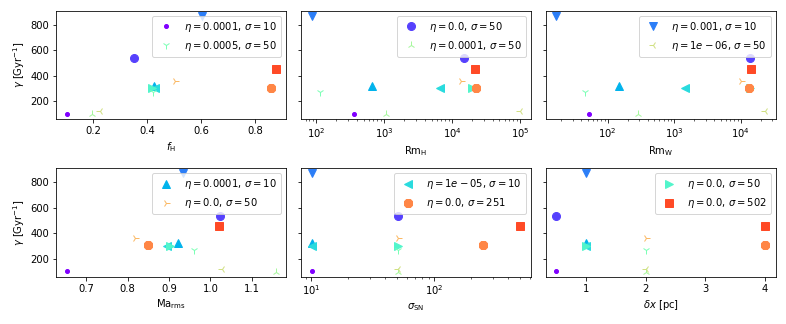
\includegraphics[trim=0cm 0cm 0cm 0cm,clip=true,width=1.\textwidth]{csc_figs/sim_higammas.png}
%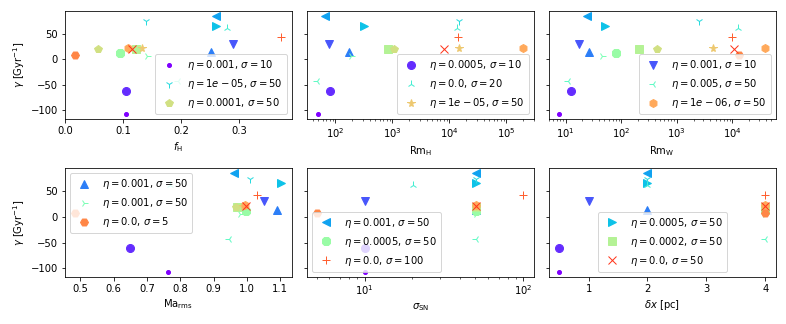
\includegraphics[trim=0cm 0cm 0cm 0cm,clip=true,width=1.\textwidth]{csc_figs/sim_gammas.png}
%\caption{
%Growth rate dependence on fractional volume of hot gas, $f_H$, magnetic Reynolds
%number in the hot and warm gas, Rm$_{\rm H}$ and Rm$_{\rm W}$, respectively, 
%Ma$_{\rm rms}$,  $u_{\rm rms}$ and resolution.
%Top panels show models during growth rates, $\gamma>100$\,Gyr$^{-1}$ and 
%bottom panels for lower growth rates.
%\label{fig:sim_gamma}
%}
%\end{figure*}
%%--------------------------------------------------------------------------

%--------------------------------------------------------------------------

For the models with 4 parsec resolution the mimimum coefficient for the 
6th order hyper diffusion is $2\cdot10^{-12}\,{\rm kpc\,km\,s}^{-1}$ to
resolve the smallest scales of the magnetic field.
The simulation with only hyper diffusion applying for the momentum, energy and
induction equations and shock capturing diffusivity for the momentum, energy and
continuity equations is continued with various constant $\nu=\eta$.
${\rm Pm}=1$ is tested first, to identify a minimum below which only the
hyper diffusion is effective.

For ${\rm Pm}>1$ tests resulted in inconsistent dynamo amplification.
Also, a set of solutions for ${\rm Pm}=1$, where the SN were applied 
independently yielded inconssitent growth rates, and the models plotted here
took applied the same incidence and location of SN as in the original 
simulation.
In the independent set of runs, only $\nu=5\cdot10^{-5}$ yielded a growth rate
similar to the original simulation, while all others exhibited stronger
amplification than obtained here.
Perhaps the increased strength of the turbulence due to the random effects of
the SN forcing, explains the enhanced growth rate for the magnetic field.

The model with the fastest growth for 4 parsec resolution has a much hotter 
domain, with the cool dense region confined to a small clump, compared to the
other models.
The increased turbulence may be a physical perturbation due to the random 
forcing, but coudl also be overheating due to numerical errors at this coarse
resolution. 
The 2 parsec resolution runs, give a more consistent response even when 
different Prandtl numbers apply.
The ${\rm Pm}=1$ runs are still running, but an example with the mixed Pm is
included.
The slices for the 2 pc resolution are obtained with ${\cal D}_3=6.25\cdot
10^{-14}$, which appears to be slightly under resolving the magnetic
field in the high Pm models. So, the subsequent
runs are applying ${\cal D}_3=8.25\cdot
10^{-14}$, allowing for the velocity extrema to have higher magnitudes
than at 4 pc
resolution.

%-----------------------------------------------------------------------------
\section*{Acknowledgements}
%-----------------------------------------------------------------------------
  Financial support from the Academy of Finland Centre of Excellence ReSoLVE 
  (project number 272157) is acknowledged (FAG); 
  Support: Grand Challenge project SNDYN, CSC-IT Center for Science Ltd. (FAG); 
%------------------------------------------------------------------------- 
\bibliographystyle{aasjournal}
\bibliography{refs}{}

\newpage 

%-------------------------------------------------------------------------
\appendix
%-------------------------------------------------------------------------

\section*{simulation notes}

\begin{table*}
\caption{\texttt{*} indicates simulation data lost}
\begin{tabular}{lccccccc}
Model & resolution & $\eta_3,\nu_3$ & $\nu$ & $\eta$ & $\sigma_{\rm SN}$ & \\
\texttt{05pc\_01SNseed*} & 0.5 & 3.25$\cdot10^{-16}$ &                  &                 &  5   \\
\texttt{05pc\_h5seed  }  & 0.5 & 3.25$\cdot10^{-16}$ &                  &                 &  50  \\
\texttt{05pcPm0e-3.0 }   & 0.5 & 3.25$\cdot10^{-16}$ &                  & $     10^{-3}$  &  10  \\
\texttt{05pcPm0e-3.3 }   & 0.5 & 3.25$\cdot10^{-16}$ &                  & 5$\cdot10^{-3}$ &  10  \\
\texttt{05pcPm0e-4.0 }   & 0.5 & 3.25$\cdot10^{-16}$ &                  & $     10^{-4}$  &  10  \\
\texttt{1pc\_01SNseed*}  & 1.0 & 3.5$\cdot10^{-15}$  &                  &                 &  20  \\
\texttt{1pc\_h5seed   }  & 1.0 & 3.5$\cdot10^{-15}$  &                  &                 &  50  \\
\texttt{1pcPm0e-3.0  }   & 1.0 & 3.5$\cdot10^{-15}$  &                  & $     10^{-3}$  &  10  \\
\texttt{1pcPm0e-4.0  }   & 1.0 & 3.5$\cdot10^{-15}$  &                  & $     10^{-4}$  &  10  \\
\texttt{1pcPm0e-5.0  }   & 1.0 & 3.5$\cdot10^{-15}$  &                  & $     10^{-5}$  &  10  \\
\texttt{1pcPm1n-4.0* }   & 1.0 & 3.5$\cdot10^{-15}$  & $     10^{-4}$   & $     10^{-4}$  &  50  \\
\texttt{1pcPm1n-5.0* }   & 1.0 & 3.5$\cdot10^{-15}$  & $     10^{-5}$   & $     10^{-5}$  &  50  \\
\texttt{2pc\_01SNseed }  & 2.0 & 8.25$\cdot10^{-14}$ &                  &                 &  20  \\
\texttt{2pc\_h5seed   }  & 2.0 & 8.25$\cdot10^{-14}$ &                  &                 &  50  \\
\texttt{2pcPm0e-3.0  }   & 2.0 & 8.25$\cdot10^{-14}$ &                  & $     10^{-3}$  &  50  \\
\texttt{2pcPm0e-3.3  }   & 2.0 & 8.25$\cdot10^{-14}$ &                  & 5$\cdot10^{-4}$ &  50  \\
\texttt{2pcPm0e-4.0  }   & 2.0 & 8.25$\cdot10^{-14}$ &                  & $     10^{-4}$  &  50  \\
\texttt{2pcPm0e-5.0  }   & 2.0 & 8.25$\cdot10^{-14}$ &                  & $     10^{-5}$  &  50  \\
\texttt{2pcPm0e-6.0  }   & 2.0 & 8.25$\cdot10^{-14}$ &                  & $     10^{-6}$  &  50  \\
\texttt{2pcPm1n-3.0* }   & 2.0 & 8.25$\cdot10^{-14}$ & $     10^{-3}$   & $     10^{-3}$  &  50  \\
\texttt{2pcPm1n-3.3  }   & 2.0 & 8.25$\cdot10^{-14}$ & 5$\cdot10^{-4}$  & 5$\cdot10^{-4}$ &  50  \\
\texttt{4pc\_01SNseed }  & 4.0 & 2$\cdot10^{-12}$    &                  &                 &  5   \\
\texttt{4pc\_h5seed   }  & 4.0 & 2$\cdot10^{-12}$    &                  &                 &  50  \\
\texttt{4pc\_2SNseed  }  & 4.0 & 2$\cdot10^{-12}$    &                  &                 & 100  \\
\texttt{4pc\_5SNseed  }  & 4.0 & 2$\cdot10^{-12}$    &                  &                 & 250  \\
\texttt{4pc\_cst5SNseed*}& 4.0 & 2$\cdot10^{-12}$    &                  &                 & 250  \\
\texttt{4pc\_10SNseed }  & 4.0 & 2$\cdot10^{-12}$    &                  &                 & 500  \\
\texttt{4pcPm0e-3.3  }   & 4.0 & 2$\cdot10^{-12}$    &                  & 5$\cdot10^{-3}$ &  50  \\
\texttt{4pcPm0e-3.0  }   & 4.0 & 2$\cdot10^{-12}$    &                  & $     10^{-3}$  &  50  \\
\texttt{4pcPm0e-3.3  }   & 4.0 & 2$\cdot10^{-12}$    &                  & 5$\cdot10^{-4}$ &  50  \\
\texttt{4pcPm0e-3.7  }   & 4.0 & 2$\cdot10^{-12}$    &                  & 2$\cdot10^{-4}$ &  50  \\
\texttt{4pcPm0e-4.0  }   & 4.0 & 2$\cdot10^{-12}$    &                  & $     10^{-4}$  &  50  \\
\texttt{4pcPm0e-5.0  }   & 4.0 & 2$\cdot10^{-12}$    &                  & $     10^{-5}$  &  50  \\
\texttt{4pcPm0e-6.0  }   & 4.0 & 2$\cdot10^{-12}$    &                  & $     10^{-6}$  &  50  \\
\texttt{4pcPm1n-2.3  }   & 4.0 & 2$\cdot10^{-12}$    & 5$\cdot10^{-3}$  & 5$\cdot10^{-3}$ &  50  \\
\texttt{4pcPm1n-3.7}     & 4.0 & 2$\cdot10^{-12}$    & 2$\cdot10^{-4}$  & 2$\cdot10^{-4}$ &  50    
\end{tabular}
\end{table*}

Next meeting mon 24/2/2020 18:30 (FI)
\begin{itemize} 
\item compare thermal runaway with Li \& Ostriker 
\item check $\gamma$ for high $\sigma_{\rm sn}$ at 4pc resolution
\item check $\gamma$ for low $\sigma_{\rm sn}$ at high resolution
\item use $\nu = 0$ to avoid changes to flow dynamics
\item check $B_0\exp(\gamma t): \gamma\propto R_{\rm m}$
\end{itemize} 

Next meeting mon 2/3/2020 17:00 (FI)
\begin{itemize} 
\item compare varying eta across resolution for physical Rm 
\item is critical value of $10^{-4}, 10^{-3}$ repeated at high resolution
\item compare separately $\gamma$ for thermal runaway vs non-thermal runaway
\item $R_{\rm m}$ within 10 zones applies $<10^{-5}$ from hyper diffusion
\end{itemize} 

Next meeting Wed 11/3/2020 16:00 (FI)
\begin{itemize} 
\item 2D histograms/pdfs of entropy vs magnetic energy
\item include spectra during growth with time evolution (hot vs cold)
\item use auto-correlation functions to determine typical velocity per phase
\item see Chira et al / Mac Low
\item test $B_0\exp(\gamma t): \gamma\propto R_{\rm m}$
\end{itemize} 

Next meeting Tue 17/3/2020 16:00 (FI)
\begin{itemize} 
\item 2D histograms/pdfs of entropy vs magnetic energy
\item include spectra during growth with time evolution (hot vs cold)
\item use auto-correlation functions to determine typical velocity per phase
\item see Chira et al / Mac Low
\item test $B_0\exp(\gamma t): \gamma\propto R_{\rm m}$
\item fix Pm calculation nu/eta not Rm/Re
\item Compare hot fraction and Rm between growth rate transition in 1pc and 2pc runs
\item Confirm whether numerical resistivity is not dominant at 1pc and 2pc runs for $\eta=10^{-4}$
\end{itemize} 

Next meeting Tue 24/3/2020 16:00 (FI)
\begin{itemize} 
\item include spectra during growth with time evolution (hot vs cold)
\item use auto-correlation functions to determine typical velocity per phase
\item see Chira et al / Mac Low
\item test $B_0\exp(\gamma t): \gamma\propto R_{\rm m}$
\item Compare hot fraction and Rm between growth rate transition in 1pc and 2pc runs
\item Confirm whether numerical resistivity is not dominant at 1pc and 2pc runs for $\eta=10^{-4}$
\item 
\end{itemize} 

Next meeting Tue 31/3/2020 17:00 (FI)
\begin{itemize} 
\item use auto-correlation functions to determine typical velocity per phase
\item see Chira et al / Mac Low
\item test $B_0\exp(\gamma t): \gamma\propto R_{\rm m}$
\item Confirm whether numerical resistivity is not dominant at 1pc and 2pc runs for $\eta=10^{-4}$
\item Run 2 and 4 pc with $\sigma_{\rm sn}=10$ and $\eta=10^{-3}$ for comparison
\item Investigate behaviour in hot gas for fast runs -- is there a slow
dynamo in warm gas and fast dynamo in hot gas
\item Scale of dynamo forcing may not be the scale of the SN bubbles? Peak of magnetic energy spectrum may be the relevant scale
\item Compare peak $k$ of $P_B(k)$, is $\eta\propto\ell^2$?
\item $k^{3/2}$ not obeyed at low $k$ - does this correspond to bubble size? Auto-correlation analysis to compare $\ell$ with bubble size $L_{\rm SN}$ and $k$-space.
\item At low Ma forcing scale determines dynamo Rm, while for high Ma does
Rm scale match $P_B(k)$ peak?
\item start experiments with explicit viscosity.
\end{itemize} 

Next meeting Tue 7/4/2020 17:00 (FI)
\begin{itemize} 
\item apply Helmholtz decomposition to the total flow. Compare vorticity in hot
phase prior to and during the dynamo epoch. Is there a jump in vorticity in the
hot gas? How is this evolving in the warm gas related to the dynamo state? 
Vorticity has been demonstrated to strongly affect SSD in other systems.
\item Investigate behaviour in hot gas for fast runs -- is there a slow
dynamo in warm gas and fast dynamo in hot gas. Plot evolution of magentic energy
density separately for the hot gas and warm gas.
\item use auto-correlation functions to determine typical velocity per phase.
Does James' method account for the discontinuous volume of the hot gas to
recover the relevant correlation length by phase? Check references/Anvar?
Divide out volume correlation function from correlation function of phase?
\item $k^{3/2}$ not obeyed at low $k$ - does this correspond to bubble size?
Auto-correlation analysis to compare $\ell$ with bubble size $L_{\rm SN}$
and $k$-space.
Power laws fit well for magnetic but not kinetic.
Is this due to two dynamos?
Separate hot amd warm gas to investigate spectra and auto-correlation.
\item see Chira et al / Mac Low
\item test $B_0\exp(\gamma t): \gamma\propto R_{\rm m}$
\item Confirm whether numerical resistivity is not dominant at 1pc and 2pc runs for $\eta=10^{-4}$
\item Scale of dynamo forcing may not be the scale of the SN bubbles? Peak of magnetic energy spectrum may be the relevant scale
\item Compare peak $k$ of $P_B(k)$, is $\eta\propto\ell^2$?
\item At low Ma forcing scale determines dynamo Rm, while for high Ma does
Rm scale match $P_B(k)$ peak?
\item start experiments with explicit viscosity.
\end{itemize} 

Update 19th May 2020 - summary of hypotheses
\begin{itemize}
\item Do the kinetic power spectra follow 5/3 power law? 
\item correlation functions - divide out corr function by volume to obtain phase?
\item Relation between Pm and Rm is counter intuitive, what about the differences in length scale between the ISM phases?
\item in the saturated state the kinetic energy matters, but in the kinematic phase purely $u^2$ may be significant even for the hot gas.
\item Is there a change in the energy at the point where the hot phase starts growing 
\item decompose the Mach number by phase to indicate level of compressibility.
\item decompose magnetic energy by phase
\item include error bars for variance of orthogonality by point
\item what is the error in div/curl
\item apply test flows to Helmholtz decomposition
\item smmothing of flow did not resolve discrepencies.
\item Is warm $e_B$ growth accummulation from hot dynamo? - delay in time? - growth of warm Ma during dynamo?
\item Drop in hot Ma during dynamo 0.04 Gyr 1pcPm0e-3. 
\item 1pcPm0e-4 Check if sudden heating coincides with growth 0.02 -0.04 vs 0.04-0.045
\item Is energy growing in warm or hot ISM?
\item check Rm for a particular location and check Rm is correct.
\end{itemize}


%------------------------------------------------------------------------
\begin{figure*}
\centering
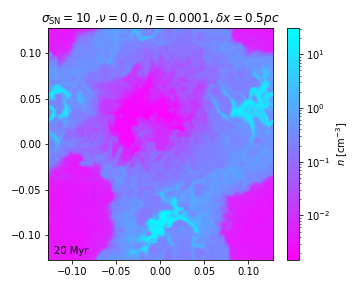
\includegraphics[trim=0.0cm 0.00cm 0.0cm 0.0cm,clip=true,width=0.33\textwidth]{csc_figs/rho05pcPm0e-4_02.png}
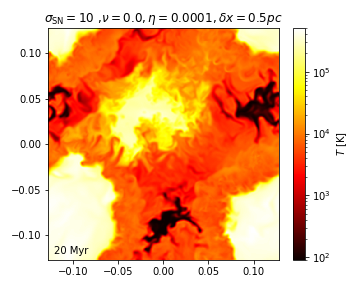
\includegraphics[trim=0.0cm 0.00cm 0.0cm 0.0cm,clip=true,width=0.33\textwidth]{csc_figs/tt05pcPm0e-4_02.png}
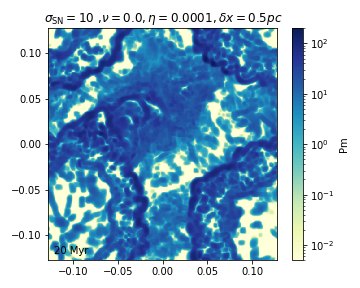
\includegraphics[trim=0.0cm 0.00cm 0.0cm 0.0cm,clip=true,width=0.33\textwidth]{csc_figs/Pm05pcPm0e-4_02.png}
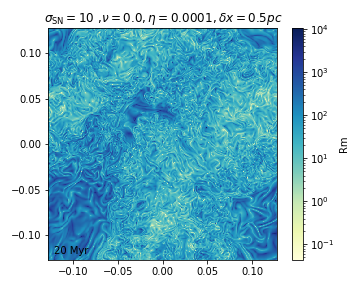
\includegraphics[trim=0.0cm 0.00cm 0.0cm 0.0cm,clip=true,width=0.33\textwidth]{csc_figs/Rm05pcPm0e-4_02.png}
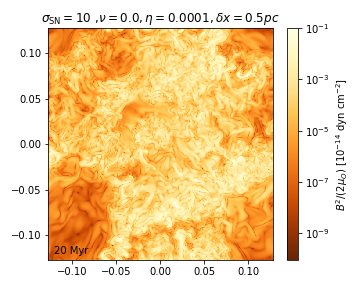
\includegraphics[trim=0.0cm 0.00cm 0.0cm 0.0cm,clip=true,width=0.33\textwidth]{csc_figs/pb05pcPm0e-4_02.png}
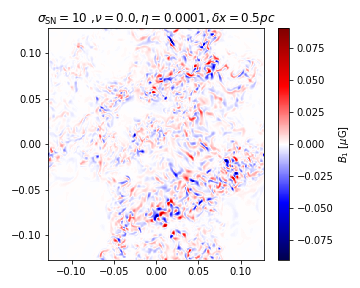
\includegraphics[trim=0.0cm 0.00cm 0.0cm 0.0cm,clip=true,width=0.33\textwidth]{csc_figs/bb105pcPm0e-4_02.png}
\caption{
Slices for resolution of 0.5\,pc with hyper diffusion coefficients as 
specified in Figure\,\ref{fig:brms}, and $\eta=10^{-4}$ sampled from the 
kinematic dynamo state.
\label{fig:05pcUB}
}
\end{figure*}
%--------------------------------------------------------------------------

%------------------------------------------------------------------------
\begin{figure*}
\centering
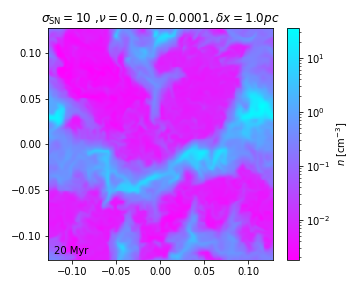
\includegraphics[trim=0.0cm 0.00cm 0.0cm 0.0cm,clip=true,width=0.33\textwidth]{csc_figs/rho1pcPm0e-4_00.png}
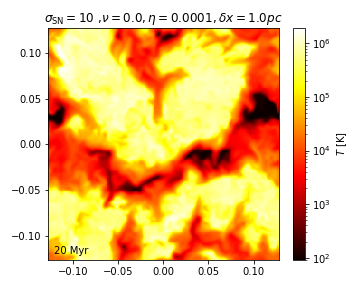
\includegraphics[trim=0.0cm 0.00cm 0.0cm 0.0cm,clip=true,width=0.33\textwidth]{csc_figs/tt1pcPm0e-4_00.png}
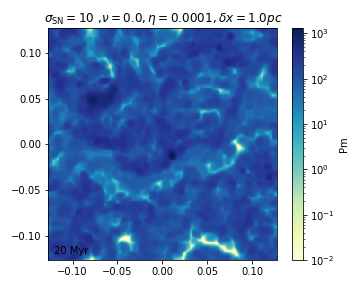
\includegraphics[trim=0.0cm 0.00cm 0.0cm 0.0cm,clip=true,width=0.33\textwidth]{csc_figs/Pm1pcPm0e-4_00.png}
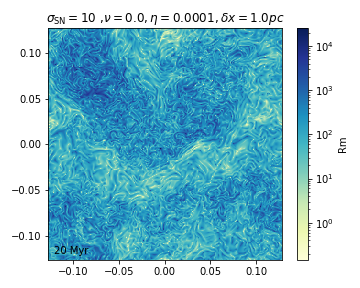
\includegraphics[trim=0.0cm 0.00cm 0.0cm 0.0cm,clip=true,width=0.33\textwidth]{csc_figs/Rm1pcPm0e-4_00.png}
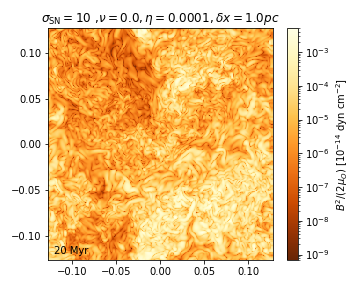
\includegraphics[trim=0.0cm 0.00cm 0.0cm 0.0cm,clip=true,width=0.33\textwidth]{csc_figs/pb1pcPm0e-4_00.png}
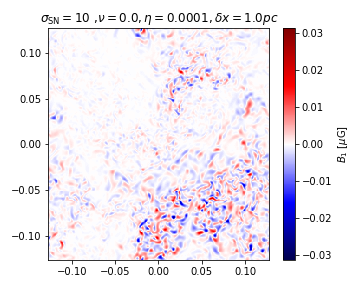
\includegraphics[trim=0.0cm 0.00cm 0.0cm 0.0cm,clip=true,width=0.33\textwidth]{csc_figs/bb11pcPm0e-4_00.png}
\caption{
Slices for resolution of 1\,pc with hyper diffusion coefficients as 
specified in Figure\,\ref{fig:brms}, and $\eta=10^{-4}$ sampled from the 
kinematic dynamo state.
\label{fig:1pcUB}
}
\end{figure*}
%--------------------------------------------------------------------------

%-------------------------------------------------------------------------
\begin{figure*}
\centering
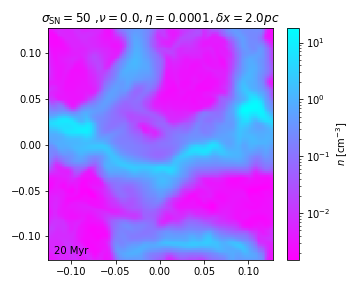
\includegraphics[trim=0.0cm 0.00cm 0.0cm 0.0cm,clip=true,width=0.33\textwidth]{csc_figs/rho2pcPm0e-4_00.png}
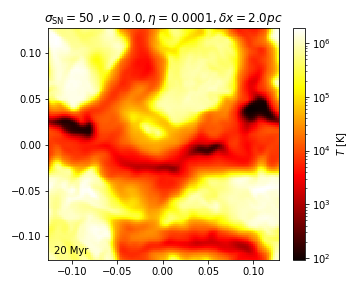
\includegraphics[trim=0.0cm 0.00cm 0.0cm 0.0cm,clip=true,width=0.33\textwidth]{csc_figs/tt2pcPm0e-4_00.png}
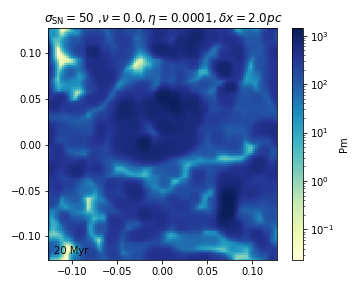
\includegraphics[trim=0.0cm 0.00cm 0.0cm 0.0cm,clip=true,width=0.33\textwidth]{csc_figs/Pm2pcPm0e-4_00.png}
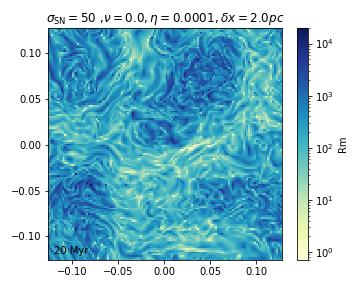
\includegraphics[trim=0.0cm 0.00cm 0.0cm 0.0cm,clip=true,width=0.33\textwidth]{csc_figs/Rm2pcPm0e-4_00.png}
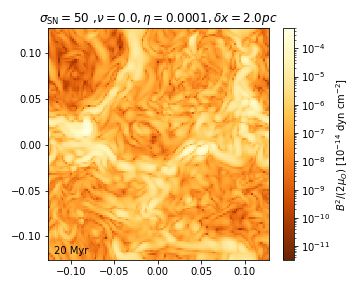
\includegraphics[trim=0.0cm 0.00cm 0.0cm 0.0cm,clip=true,width=0.33\textwidth]{csc_figs/pb2pcPm0e-4_00.png}
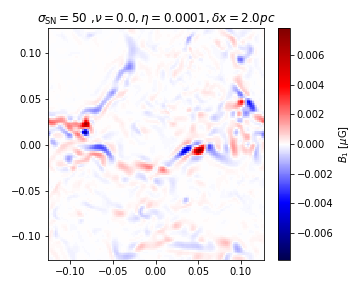
\includegraphics[trim=0.0cm 0.00cm 0.0cm 0.0cm,clip=true,width=0.33\textwidth]{csc_figs/bb12pcPm0e-4_00.png}
\caption{
Slices for resolution of 2\,pc with hyper diffusion coefficients as 
specified in Figure\,\ref{fig:brms}, and $\eta=10^{-4}$ sampled from the 
kinematic dynamo state.
\label{fig:2pcUB}
}
\end{figure*}
%--------------------------------------------------------------------------

%-------------------------------------------------------------------------
\begin{figure*}
\centering
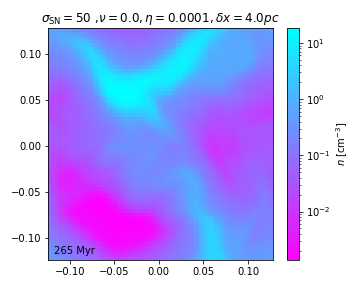
\includegraphics[trim=0.0cm 0.00cm 0.0cm 0.0cm,clip=true,width=0.33\textwidth]{csc_figs/rho4pcPm0e-4_032.png}
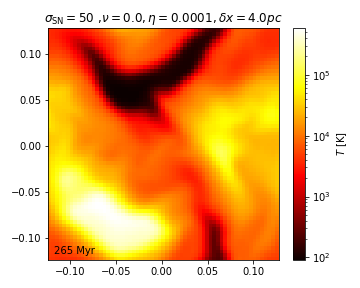
\includegraphics[trim=0.0cm 0.00cm 0.0cm 0.0cm,clip=true,width=0.33\textwidth]{csc_figs/tt4pcPm0e-4_032.png}
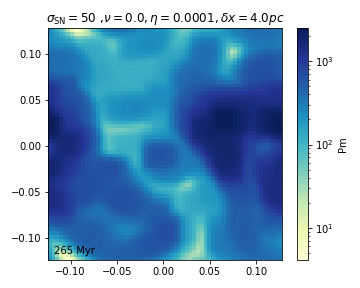
\includegraphics[trim=0.0cm 0.00cm 0.0cm 0.0cm,clip=true,width=0.33\textwidth]{csc_figs/Pm4pcPm0e-4_032.png}
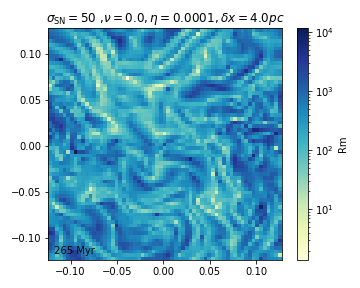
\includegraphics[trim=0.0cm 0.00cm 0.0cm 0.0cm,clip=true,width=0.33\textwidth]{csc_figs/Rm4pcPm0e-4_032.png}
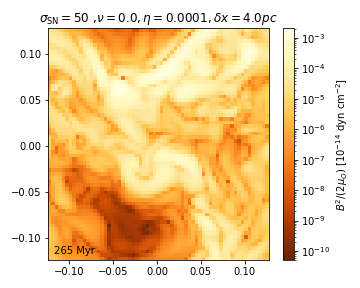
\includegraphics[trim=0.0cm 0.00cm 0.0cm 0.0cm,clip=true,width=0.33\textwidth]{csc_figs/pb4pcPm0e-4_032.png}
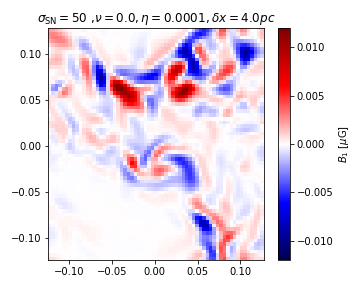
\includegraphics[trim=0.0cm 0.00cm 0.0cm 0.0cm,clip=true,width=0.33\textwidth]{csc_figs/bb14pcPm0e-4_032.png}
\caption{
Slices for resolution of 4\,pc with hyper diffusion coefficients as 
specified in Figure\,\ref{fig:brms}, and $\eta=10^{-4}$ sampled from the 
kinematic dynamo state.
\label{fig:4pcUB}
}
\end{figure*}
%--------------------------------------------------------------------------

%-------------------------------------------------------------------------
\begin{figure*}
\centering
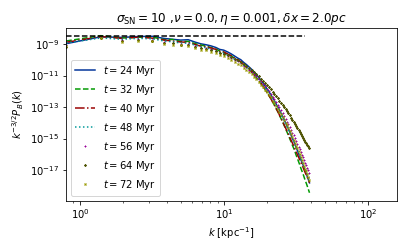
\includegraphics[trim=0.0cm 0.00cm 0.0cm 0.0cm,clip=true,width=0.45\textwidth]{csc_figs/2pcPm0e-3_02SNBpower.png}
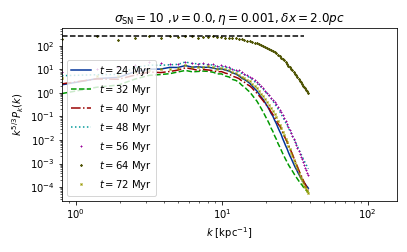
\includegraphics[trim=0.0cm 0.00cm 0.0cm 0.0cm,clip=true,width=0.45\textwidth]{csc_figs/2pcPm0e-3_02SNkpower.png}
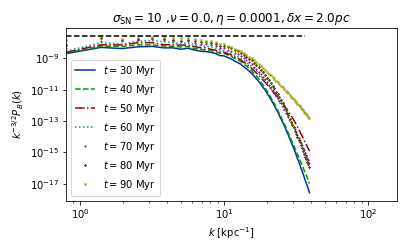
\includegraphics[trim=0.0cm 0.00cm 0.0cm 0.0cm,clip=true,width=0.45\textwidth]{csc_figs/2pcPm0e-4_02SNBpower.png}
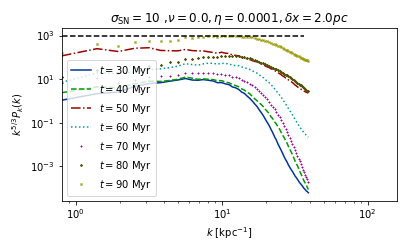
\includegraphics[trim=0.0cm 0.00cm 0.0cm 0.0cm,clip=true,width=0.45\textwidth]{csc_figs/2pcPm0e-4_02SNkpower.png}
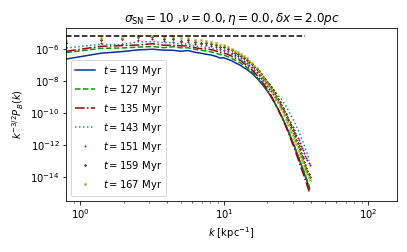
\includegraphics[trim=0.0cm 0.00cm 0.0cm 0.0cm,clip=true,width=0.45\textwidth]{csc_figs/2pcPm0e-0_02SNBpower.png}
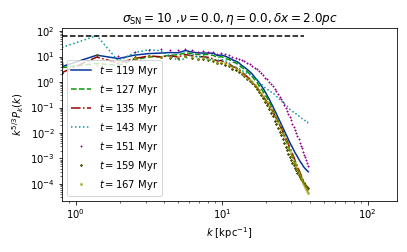
\includegraphics[trim=0.0cm 0.00cm 0.0cm 0.0cm,clip=true,width=0.45\textwidth]{csc_figs/2pcPm0e-0_02SNkpower.png}
\caption{
Magnetic (left) and kinetic (right) energy spectra for 2pc resolution runs 
during the kinematic growth phases with ${\cal D}_3$ 
coefficients as specified in Figure\,\ref{fig:brms}, and $\eta\in[0,10^{-3}]$.
$\sigma_{\rm SN}=10$.
\label{fig:2spectra10SN}
}
\end{figure*}
%--------------------------------------------------------------------------


%-------------------------------------------------------------------------
\begin{figure*}
\centering
\includegraphics[trim=0.0cm 0.00cm 0.0cm 0.0cm,clip=true,width=0.45\textwidth]{csc_figs/4pcPm0e-3_02SNBpower.png}
\includegraphics[trim=0.0cm 0.00cm 0.0cm 0.0cm,clip=true,width=0.45\textwidth]{csc_figs/4pcPm0e-3_02SNkpower.png}
\includegraphics[trim=0.0cm 0.00cm 0.0cm 0.0cm,clip=true,width=0.45\textwidth]{csc_figs/4pcPm0e-4_02SNBpower.png}
\includegraphics[trim=0.0cm 0.00cm 0.0cm 0.0cm,clip=true,width=0.45\textwidth]{csc_figs/4pcPm0e-4_02SNkpower.png}
\includegraphics[trim=0.0cm 0.00cm 0.0cm 0.0cm,clip=true,width=0.45\textwidth]{csc_figs/4pcPm0e-0_02SNBpower.png}
\includegraphics[trim=0.0cm 0.00cm 0.0cm 0.0cm,clip=true,width=0.45\textwidth]{csc_figs/4pcPm0e-0_02SNkpower.png}
\caption{
Magnetic (left) and kinetic (right) energy spectra for 4pc resolution runs 
during the kinematic growth phases with ${\cal D}_3$ 
coefficients as specified in Figure\,\ref{fig:brms}, and $\eta\in[0,10^{-3}]$.
$\sigma_{\rm SN}=10$.
\label{fig:4spectra10SN}
}
\end{figure*}
%--------------------------------------------------------------------------


%-------------------------------------------------------------------------
\begin{figure*}
\centering
\includegraphics[trim=0.0cm 0.00cm 0.0cm 0.0cm,clip=true,width=0.45\textwidth]{csc_figs/05pcPm0e-4_0Bpower.png}
\includegraphics[trim=0.0cm 0.00cm 0.0cm 0.0cm,clip=true,width=0.45\textwidth]{csc_figs/05pcPm0e-4_0kpower.png}
\includegraphics[trim=0.0cm 0.00cm 0.0cm 0.0cm,clip=true,width=0.45\textwidth]{csc_figs/1pcPm0e-4_0Bpower.png}
\includegraphics[trim=0.0cm 0.00cm 0.0cm 0.0cm,clip=true,width=0.45\textwidth]{csc_figs/1pcPm0e-4_0kpower.png}
\includegraphics[trim=0.0cm 0.00cm 0.0cm 0.0cm,clip=true,width=0.45\textwidth]{csc_figs/2pcPm0e-4_0Bpower.png}
\includegraphics[trim=0.0cm 0.00cm 0.0cm 0.0cm,clip=true,width=0.45\textwidth]{csc_figs/2pcPm0e-4_0kpower.png}
\includegraphics[trim=0.0cm 0.00cm 0.0cm 0.0cm,clip=true,width=0.45\textwidth]{csc_figs/4pcPm0e-4_0Bpower.png}
\includegraphics[trim=0.0cm 0.00cm 0.0cm 0.0cm,clip=true,width=0.45\textwidth]{csc_figs/4pcPm0e-4_0kpower.png}
\caption{
Magnetic (left) and kinetic (right) energy spectra for all resolution runs 
during the kinematic growth phases with ${\cal D}_3$ 
coefficients as specified in Figure\,\ref{fig:brms}, and $\eta=10^{-4}$.
$\sigma_{\rm SN}=10$ at higher resolution and $\sigma_{\rm SN}=50$ for lower
resolution.
\label{fig:4spectraRm}
}
\end{figure*}
%--------------------------------------------------------------------------

%-------------------------------------------------------------------------
\begin{figure*}
\centering
\includegraphics[trim=0.0cm 0.00cm 0.0cm 0.0cm,clip=true,width=0.45\textwidth]{csc_figs/05pcPm0e-3_0Bpower.png}
\includegraphics[trim=0.0cm 0.00cm 0.0cm 0.0cm,clip=true,width=0.45\textwidth]{csc_figs/05pcPm0e-3_0kpower.png}
\includegraphics[trim=0.0cm 0.00cm 0.0cm 0.0cm,clip=true,width=0.45\textwidth]{csc_figs/05pcPm0e-3_3Bpower.png}
\includegraphics[trim=0.0cm 0.00cm 0.0cm 0.0cm,clip=true,width=0.45\textwidth]{csc_figs/05pcPm0e-3_3kpower.png}
\includegraphics[trim=0.0cm 0.00cm 0.0cm 0.0cm,clip=true,width=0.45\textwidth]{csc_figs/05pcPm0e-4_0Bpower.png}
\includegraphics[trim=0.0cm 0.00cm 0.0cm 0.0cm,clip=true,width=0.45\textwidth]{csc_figs/05pcPm0e-4_0kpower.png}
\caption{
Magnetic (left) and kinetic (right) energy spectra for 0.5\,pc resolution runs 
during the kinematic growth phases with ${\cal D}_3$ 
coefficients as specified in Figure\,\ref{fig:brms}, and $\eta\in[10^{-3},10^{-4}]$. $\sigma_{\rm SN}=10$.
\label{fig:4spectraRm}
}
\end{figure*}
%--------------------------------------------------------------------------

%-------------------------------------------------------------------------
\begin{figure*}
\centering
\includegraphics[trim=0.0cm 0.00cm 0.0cm 0.0cm,clip=true,width=0.45\textwidth]{csc_figs/1pcPm0e-3_0Bpower.png}
\includegraphics[trim=0.0cm 0.00cm 0.0cm 0.0cm,clip=true,width=0.45\textwidth]{csc_figs/1pcPm0e-3_0kpower.png}
\includegraphics[trim=0.0cm 0.00cm 0.0cm 0.0cm,clip=true,width=0.45\textwidth]{csc_figs/1pcPm0e-4_0Bpower.png}
\includegraphics[trim=0.0cm 0.00cm 0.0cm 0.0cm,clip=true,width=0.45\textwidth]{csc_figs/1pcPm0e-4_0kpower.png}
\includegraphics[trim=0.0cm 0.00cm 0.0cm 0.0cm,clip=true,width=0.45\textwidth]{csc_figs/1pcPm0e-5_0Bpower.png}
\includegraphics[trim=0.0cm 0.00cm 0.0cm 0.0cm,clip=true,width=0.45\textwidth]{csc_figs/1pcPm0e-5_0kpower.png}
\caption{
Magnetic (left) and kinetic (right) energy spectra for 1\,pc resolution runs 
during the kinematic growth phases with ${\cal D}_3$ 
coefficients as specified in Figure\,\ref{fig:brms}, and $\eta\in[10^{-3},10^{-5}]$. $\sigma_{\rm SN}=10$.
\label{fig:4spectraRm}
}
\end{figure*}
%--------------------------------------------------------------------------

%-------------------------------------------------------------------------
\begin{figure*}
\centering
\includegraphics[trim=0.0cm 0.00cm 0.0cm 0.0cm,clip=true,width=0.45\textwidth]{csc_figs/2pcPm0e-3_0Bpower.png}
\includegraphics[trim=0.0cm 0.00cm 0.0cm 0.0cm,clip=true,width=0.45\textwidth]{csc_figs/2pcPm0e-3_0kpower.png}
\includegraphics[trim=0.0cm 0.00cm 0.0cm 0.0cm,clip=true,width=0.45\textwidth]{csc_figs/2pcPm0e-3_aBpower.png}
\includegraphics[trim=0.0cm 0.00cm 0.0cm 0.0cm,clip=true,width=0.45\textwidth]{csc_figs/2pcPm0e-3_akpower.png}
\includegraphics[trim=0.0cm 0.00cm 0.0cm 0.0cm,clip=true,width=0.45\textwidth]{csc_figs/2pcPm0e-3_3Bpower.png}
\includegraphics[trim=0.0cm 0.00cm 0.0cm 0.0cm,clip=true,width=0.45\textwidth]{csc_figs/2pcPm0e-3_3kpower.png}
\includegraphics[trim=0.0cm 0.00cm 0.0cm 0.0cm,clip=true,width=0.45\textwidth]{csc_figs/2pcPm0e-3_bBpower.png}
\includegraphics[trim=0.0cm 0.00cm 0.0cm 0.0cm,clip=true,width=0.45\textwidth]{csc_figs/2pcPm0e-3_bkpower.png}
\caption{
Magnetic (left) and kinetic (right) energy spectra for 2\,pc resolution runs 
showing change in Kolmogorov scaling between
 the low and high kinematic growth phases with ${\cal D}_3$ 
coefficients as specified in Figure\,\ref{fig:brms}, and $\eta\in[5\cdot10^{-3},10^{-3}]$. $\sigma_{\rm SN}=50$.
\label{fig:4spectraRm}
}
\end{figure*}
%--------------------------------------------------------------------------

%-------------------------------------------------------------------------
\begin{figure*}
\centering
\includegraphics[trim=0.0cm 0.00cm 0.0cm 0.0cm,clip=true,width=0.45\textwidth]{csc_figs/4pcPm0e-2_3Bpower.png}
\includegraphics[trim=0.0cm 0.00cm 0.0cm 0.0cm,clip=true,width=0.45\textwidth]{csc_figs/4pcPm0e-2_3kpower.png}
\includegraphics[trim=0.0cm 0.00cm 0.0cm 0.0cm,clip=true,width=0.45\textwidth]{csc_figs/4pcPm0e-3_0Bpower.png}
\includegraphics[trim=0.0cm 0.00cm 0.0cm 0.0cm,clip=true,width=0.45\textwidth]{csc_figs/4pcPm0e-3_0kpower.png}
\includegraphics[trim=0.0cm 0.00cm 0.0cm 0.0cm,clip=true,width=0.45\textwidth]{csc_figs/4pcPm0e-4_0Bpower.png}
\includegraphics[trim=0.0cm 0.00cm 0.0cm 0.0cm,clip=true,width=0.45\textwidth]{csc_figs/4pcPm0e-4_0kpower.png}
\includegraphics[trim=0.0cm 0.00cm 0.0cm 0.0cm,clip=true,width=0.45\textwidth]{csc_figs/4pcPm0e-5_0Bpower.png}
\includegraphics[trim=0.0cm 0.00cm 0.0cm 0.0cm,clip=true,width=0.45\textwidth]{csc_figs/4pcPm0e-5_0kpower.png}
\caption{
Magnetic (left) and kinetic (right) energy spectra for 4\,pc resolution runs 
during the kinematic growth phases with ${\cal D}_3$ 
coefficients as specified in Figure\,\ref{fig:brms}, and $\eta\in[5\cdot10^{-3},10^{-5}]$. $\sigma_{\rm SN}=50$.
\label{fig:4spectraRm}
}
\end{figure*}
%--------------------------------------------------------------------------

%-------------------------------------------------------------------------
\begin{figure*}
\centering
\includegraphics[trim=0.0cm 0.00cm 0.0cm 0.0cm,clip=true,width=0.45\textwidth]{csc_figs/4pc_01SNseedBpower.png}
\includegraphics[trim=0.0cm 0.00cm 0.0cm 0.0cm,clip=true,width=0.45\textwidth]{csc_figs/4pc_01SNseedkpower.png}
\includegraphics[trim=0.0cm 0.00cm 0.0cm 0.0cm,clip=true,width=0.45\textwidth]{csc_figs/4pc_h5seedBpower.png}
\includegraphics[trim=0.0cm 0.00cm 0.0cm 0.0cm,clip=true,width=0.45\textwidth]{csc_figs/4pc_h5seedkpower.png}
\includegraphics[trim=0.0cm 0.00cm 0.0cm 0.0cm,clip=true,width=0.45\textwidth]{csc_figs/4pc_2SNseedBpower.png}
\includegraphics[trim=0.0cm 0.00cm 0.0cm 0.0cm,clip=true,width=0.45\textwidth]{csc_figs/4pc_2SNseedkpower.png}
\includegraphics[trim=0.0cm 0.00cm 0.0cm 0.0cm,clip=true,width=0.45\textwidth]{csc_figs/4pc_5SNseedBpower.png}
\includegraphics[trim=0.0cm 0.00cm 0.0cm 0.0cm,clip=true,width=0.45\textwidth]{csc_figs/4pc_5SNseedkpower.png}
\caption{
Magnetic (left) and kinetic (right) energy spectra for 4\,pc resolution runs 
during the kinematic growth phases with ${\cal D}_3$ 
coefficients as specified in Figure\,\ref{fig:brms}, and $\eta=0$.
 $\sigma_{\rm SN}\in[5,250]$.
\label{fig:4spectraSN}
}
\end{figure*}
%--------------------------------------------------------------------------

%%-------------------------------------------------------------------------
%\begin{figure*}
%\centering
%\includegraphics[trim=0.0cm 0.00cm 0.0cm 0.0cm,clip=true,width=0.33\textwidth]{csc_figs/1pcPm0e-3_0102D.png}
%\includegraphics[trim=0.0cm 0.00cm 0.0cm 0.0cm,clip=true,width=0.33\textwidth]{csc_figs/1pcPm0e-3_a102D.png}
%\includegraphics[trim=0.0cm 0.00cm 0.0cm 0.0cm,clip=true,width=0.33\textwidth]{csc_figs/1pcPm0e-4_0102D.png}
%\includegraphics[trim=0.0cm 0.00cm 0.0cm 0.0cm,clip=true,width=0.33\textwidth]{csc_figs/1pcPm0e-5_0102D.png}
%\includegraphics[trim=0.0cm 0.00cm 0.0cm 0.0cm,clip=true,width=0.33\textwidth]{csc_figs/1pc_h5seed102D.png}
%\caption{
%Total volume probability density distributions of ISM by Rm and temperature
%during the kinematic phase for resolution of 1\,pc with hyper diffusion
%coefficients as specified in Figure\,\ref{fig:brms}, and $\eta\in[10^{-3},0]$.
% $\sigma_{\rm SN}=10$, except last panel with $\sigma_{\rm SN}=50$.
%\label{fig:12D}
%}
%\end{figure*}
%%--------------------------------------------------------------------------

%%-------------------------------------------------------------------------
%\begin{figure*}
%\centering
%\includegraphics[trim=0.0cm 0.00cm 0.0cm 0.0cm,clip=true,width=0.33\textwidth]{csc_figs/2pcPm0e-3_0102D.png}
%\includegraphics[trim=0.0cm 0.00cm 0.0cm 0.0cm,clip=true,width=0.33\textwidth]{csc_figs/2pcPm0e-3_a102D.png}
%\includegraphics[trim=0.0cm 0.00cm 0.0cm 0.0cm,clip=true,width=0.33\textwidth]{csc_figs/2pcPm0e-3_3102D.png}
%\includegraphics[trim=0.0cm 0.00cm 0.0cm 0.0cm,clip=true,width=0.33\textwidth]{csc_figs/2pcPm0e-3_b102D.png}
%\includegraphics[trim=0.0cm 0.00cm 0.0cm 0.0cm,clip=true,width=0.33\textwidth]{csc_figs/2pcPm0e-4_0102D.png}
%\includegraphics[trim=0.0cm 0.00cm 0.0cm 0.0cm,clip=true,width=0.33\textwidth]{csc_figs/2pcPm0e-5_0102D.png}
%\includegraphics[trim=0.0cm 0.00cm 0.0cm 0.0cm,clip=true,width=0.33\textwidth]{csc_figs/2pcPm0e-6_0102D.png}
%\includegraphics[trim=0.0cm 0.00cm 0.0cm 0.0cm,clip=true,width=0.33\textwidth]{csc_figs/2pc_h5seed102D.png}
%\caption{
%Total volume probability density distributions of ISM by Rm and temperature
%during the kinematic phase for resolution of 2\,pc with hyper diffusion
%coefficients as specified in Figure\,\ref{fig:brms}, and $\eta\in[10^{-3},0]$.
% $\sigma_{\rm SN}=50$.
%\label{fig:22D}
%}
%\end{figure*}
%%--------------------------------------------------------------------------



%%-------------------------------------------------------------------------
%\begin{figure*}
%\centering
%\includegraphics[trim=0.0cm 0.00cm 0.0cm 0.0cm,clip=true,width=0.33\textwidth]{csc_figs/4pcPm0e-2_3202D.png}
%\includegraphics[trim=0.0cm 0.00cm 0.0cm 0.0cm,clip=true,width=0.33\textwidth]{csc_figs/4pcPm0e-3_0362D.png}
%\includegraphics[trim=0.0cm 0.00cm 0.0cm 0.0cm,clip=true,width=0.33\textwidth]{csc_figs/4pcPm0e-3_3182D.png}
%\includegraphics[trim=0.0cm 0.00cm 0.0cm 0.0cm,clip=true,width=0.33\textwidth]{csc_figs/4pcPm0e-3_7182D.png}
%\includegraphics[trim=0.0cm 0.00cm 0.0cm 0.0cm,clip=true,width=0.33\textwidth]{csc_figs/4pcPm0e-4_0272D.png}
%\includegraphics[trim=0.0cm 0.00cm 0.0cm 0.0cm,clip=true,width=0.33\textwidth]{csc_figs/4pcPm0e-5_0302D.png}
%\includegraphics[trim=0.0cm 0.00cm 0.0cm 0.0cm,clip=true,width=0.33\textwidth]{csc_figs/4pcPm0e-6_0332D.png}
%\includegraphics[trim=0.0cm 0.00cm 0.0cm 0.0cm,clip=true,width=0.33\textwidth]{csc_figs/4pc_h5seed332D.png}
%\includegraphics[trim=0.0cm 0.00cm 0.0cm 0.0cm,clip=true,width=0.33\textwidth]{csc_figs/4pc_5SNseed082D.png}
%\caption{
%Total volume probability density distributions of ISM by Rm and temperature
%during the kinematic phase for resolution of 4\,pc with hyper diffusion
%coefficients as specified in Figure\,\ref{fig:brms}, and $\eta\in[5\cdot10^{-3},0]$.
% $\sigma_{\rm SN}=50$, except last panel with $\sigma_{\rm SN}=250$.
%\label{fig:42D}
%}
%\end{figure*}
%%--------------------------------------------------------------------------

%%-------------------------------------------------------------------------
%\begin{figure*}
%\centering
%\includegraphics[trim=0.0cm 0.00cm 0.0cm 0.0cm,clip=true,height=0.3\textwidth]{csc_figs/histRm05pcPm0e-4_0.png}
%\includegraphics[trim=0.0cm 0.00cm 0.0cm 0.0cm,clip=true,height=0.3\textwidth]{csc_figs/hfrac05pcPm0e-4_0.png}
%\includegraphics[trim=0.0cm 0.00cm 0.0cm 0.0cm,clip=true,height=0.3\textwidth]{csc_figs/Rmfrac05pcPm0e-4_0.png}
%\caption{
%Resolution 0.5\,pc: Upper panels show PDFs for split by warm and hot phases
%of the Rm and Pm during the kinematic phase and the lower panels show the
%magnetic energy, with a fit for the growth rate during the kinematic phase
%and fractional volume of the hot gas (left) and mean Rm in the hot and 
%warm phases for the model with $\eta=10^{-4}$.
%\label{fig:histRm05_4}
%}
%\end{figure*}
%%--------------------------------------------------------------------------
%
%%-------------------------------------------------------------------------
%\begin{figure*}
%\centering
%\includegraphics[trim=0.0cm 0.00cm 0.0cm 0.0cm,clip=true,height=0.3\textwidth]{csc_figs/histRm05pcPm0e-3_0.png}
%\includegraphics[trim=0.0cm 0.00cm 0.0cm 0.0cm,clip=true,height=0.3\textwidth]{csc_figs/hfrac05pcPm0e-3_0.png}
%\includegraphics[trim=0.0cm 0.00cm 0.0cm 0.0cm,clip=true,height=0.3\textwidth]{csc_figs/Rmfrac05pcPm0e-3_0.png}
%\caption{
%Resolution 0.5\,pc: Upper panels show PDFs for split by warm and hot phases
%of the Rm and Pm during the kinematic phase and the lower panels show the
%magnetic energy, with a fit for the decay rate during the kinematic phase
%and fractional volume of the hot gas (left) and mean Rm in the hot and 
%warm phases for the model with $\eta=10^{-3}$.
%\label{fig:histRm05_3}
%}
%\end{figure*}
%%--------------------------------------------------------------------------
%
%%-------------------------------------------------------------------------
%\begin{figure*}
%\centering
%\includegraphics[trim=0.0cm 0.00cm 0.0cm 0.0cm,clip=true,height=0.3\textwidth]{csc_figs/histRm1pcPm0e-4_0.png}
%\includegraphics[trim=0.0cm 0.00cm 0.0cm 0.0cm,clip=true,height=0.3\textwidth]{csc_figs/hfrac1pcPm0e-4_0.png}
%\includegraphics[trim=0.0cm 0.00cm 0.0cm 0.0cm,clip=true,height=0.3\textwidth]{csc_figs/Rmfrac1pcPm0e-4_0.png}
%\caption{
%Resolution 1\,pc: Upper panels show PDFs for split by warm and hot phases
%of the Rm and Pm during the kinematic phase and the lower panels show the
%magnetic energy, with a fit for the growth rate during the kinematic phase
%and fractional volume of the hot gas (left) and mean Rm in the hot and 
%warm phases for the model with $\eta=10^{-4}$.
%\label{fig:histRm1_4}
%}
%\end{figure*}
%%--------------------------------------------------------------------------
%
%%-------------------------------------------------------------------------
%\begin{figure*}
%\centering
%\includegraphics[trim=0.0cm 0.00cm 0.0cm 0.0cm,clip=true,height=0.3\textwidth]{csc_figs/histRm1pcPm0e-3_0.png}
%\includegraphics[trim=0.0cm 0.00cm 0.0cm 0.0cm,clip=true,height=0.3\textwidth]{csc_figs/histRm1pcPm0e-3_a.png}
%\includegraphics[trim=0.0cm 0.00cm 0.0cm 0.0cm,clip=true,height=0.3\textwidth]{csc_figs/hfrac1pcPm0e-3_0.png}
%\includegraphics[trim=0.0cm 0.00cm 0.0cm 0.0cm,clip=true,height=0.3\textwidth]{csc_figs/hfrac1pcPm0e-3_a.png}
%\caption{
%Resolution 1\,pc: Upper panels show PDFs for split by warm and hot phases
%of the Rm and Pm during the low growth kinematic phase and the middle panels
%during the high growth kinematic phase.
%The lower panels show the magnetic energy, with a fit for the growth rate 
%during each kinematic stage and the fractional volume of the hot gas.
%Mean Rm does not strongly alter between each stage.
%The model has $\eta=10^{-3}$.
%\label{fig:histRm1_3}
%}
%\end{figure*}
%%--------------------------------------------------------------------------
%
%%-------------------------------------------------------------------------
%\begin{figure*}
%\centering
%\includegraphics[trim=0.0cm 0.00cm 0.0cm 0.0cm,clip=true,height=0.3\textwidth]{csc_figs/histRm4pcPm0e-4_0.png}
%\includegraphics[trim=0.0cm 0.00cm 0.0cm 0.0cm,clip=true,height=0.3\textwidth]{csc_figs/histRm4pc_h5seed.png}
%\includegraphics[trim=0.0cm 0.00cm 0.0cm 0.0cm,clip=true,height=0.3\textwidth]{csc_figs/hfrac4pcPm0e-4_0.png}
%\includegraphics[trim=0.0cm 0.00cm 0.0cm 0.0cm,clip=true,height=0.3\textwidth]{csc_figs/hfrac4pc_10SNseed.png}
%\caption{
%Resolution 4\,pc: Upper panels show PDFs for model with $\sigma=50$ 
%split by warm and hot phases
%of the Rm and Pm during the kinematic phase and the middle panels for the
%model with $\sigma=500$.
%The lower panels show the magnetic energy for each, with a fit for the growth
%rate during the kinematic stage and the fractional volume of the hot gas.
%The models have $\eta=10^{-4}$ and 0, respectively.
%\label{fig:histRm4_SN}
%}
%\end{figure*}
%%--------------------------------------------------------------------------

\section{Helmhlotz decomposition test sample}
%-------------------------------------------------------------------------
\begin{figure*}
\centering
\includegraphics[trim=0.4cm 0.0cm 0.0cm  0.0cm,clip=true,height=0.22\textwidth]{csc_figs/helm_test1.eps}
\includegraphics[trim=1.0cm 0.0cm 0.0cm  0.0cm,clip=true,height=0.22\textwidth]{csc_figs/helm_test2.eps}
\includegraphics[trim=1.0cm 0.0cm 0.0cm  0.0cm,clip=true,height=0.22\textwidth]{csc_figs/helm_test4.eps}
\includegraphics[trim=0.4cm 0.3cm 0.2cm -0.2cm,clip=true,height=0.22\textwidth]{csc_figs/helm_hist.eps}
\includegraphics[trim=1.0cm 0.0cm 0.0cm  0.0cm,clip=true,height=0.22\textwidth]{csc_figs/helm_test3.eps}
\includegraphics[trim=1.0cm 0.0cm 0.0cm  0.0cm,clip=true,height=0.22\textwidth]{csc_figs/helm_test5.eps}
\caption{
Test flow, panel {\bf{(a)}}, comprising sum of rotational flow, panel
{\bf{(b)}}, and potential flow, panel {\bf{(c)}}, applying the Helmholtz
decomposition result in panels {\bf{(e)}} and {\bf{(f)}}.
The PDF of the ratio of decomposed internal energy summed to total internal
energy returns a $\delta$-function, indicative of orthogonal solutions.
\label{fig:helm_test}
}
\end{figure*}
%--------------------------------------------------------------------------

%-------------------------------------------------------------------------
\begin{figure*}
\centering
\includegraphics[trim=0.4cm 0.0cm 0.0cm  0.0cm,clip=true,height=0.22\textwidth]{csc_figs/helm_sim1.eps}
\includegraphics[trim=1.0cm 0.0cm 0.0cm  0.0cm,clip=true,height=0.22\textwidth]{csc_figs/helm_sim2.eps}
\includegraphics[trim=1.0cm 0.0cm 0.0cm  0.0cm,clip=true,height=0.22\textwidth]{csc_figs/helm_sim3.eps}
\includegraphics[trim=0.4cm 0.3cm 0.2cm -0.2cm,clip=true,height=0.22\textwidth]{csc_figs/helm_hsim.eps}
\includegraphics[trim=1.0cm 0.0cm 0.0cm  0.0cm,clip=true,height=0.22\textwidth]{csc_figs/helm_divu.eps}
\includegraphics[trim=1.0cm 0.0cm 0.0cm  0.0cm,clip=true,height=0.22\textwidth]{csc_figs/helm_curl.eps}
%\includegraphics[trim=1.0cm 0.0cm 0.0cm 0.0cm,clip=true,width=0.3\textwidth]{csc_figs/helm_temp.eps}
\caption{
Simulation flow, panel {\bf{(c)}}, applying the Helmholtz decomposition result
in panels {\bf{(b)}} and {\bf{(c)}}.
The non-zero divergence of the rotational portion, {\bf{(d)}}, and curl of the
potential portion, {\bf{(e)}}, indicate the extent to which the discrete 
decomposition is not orthogonal due to extreme gradients.
Temperature, {\bf{(f)}}, is included to show how these extrema align with ISM phase.
\label{fig:helm_sim}
}
\end{figure*}
%--------------------------------------------------------------------------


%-------------------------------------------------------------------------
\begin{figure*}
\centering
\includegraphics[trim=0.0cm 0.0cm 0.0cm 0.0cm,clip=true,width=0.33\textwidth]{csc_figs/efrac_hot-1e4K_pb4pcPm0e-3_3.png}
\includegraphics[trim=0.0cm 0.0cm 0.0cm 0.0cm,clip=true,width=0.33\textwidth]{csc_figs/efrac_hot-1e4K_fV4pcPm0e-3_3.png}
\includegraphics[trim=0.0cm 0.0cm 0.0cm 0.0cm,clip=true,width=0.33\textwidth]{csc_figs/efrac_hot-1e4K_Ma4pcPm0e-3_3.png}
%\includegraphics[trim=0.0cm 0.0cm 0.0cm 0.0cm,clip=true,width=0.49\textwidth]{csc_figs/efrac_hot-1e4K_e_rot_hot4pcPm0e-3_3.png}
%\includegraphics[trim=0.0cm 0.0cm 0.0cm 0.0cm,clip=true,width=0.49\textwidth]{csc_figs/efrac_hot-1e4K_e_rot_wrm4pcPm0e-3_3.png}
%\includegraphics[trim=0.0cm 0.0cm 0.0cm 0.0cm,clip=true,width=0.49\textwidth]{csc_figs/efrac_hot-1e4K_e_pot_hot4pcPm0e-3_3.png}
%\includegraphics[trim=0.0cm 0.0cm 0.0cm 0.0cm,clip=true,width=0.49\textwidth]{csc_figs/efrac_hot-1e4K_e_pot_wrm4pcPm0e-3_3.png}
\caption{
Effect of warm and hot ISM phase dynamics on dynamo with 4\,pc resolution with
$\eta=5\cdot10^{-4}$.
Time evolution in the warm and hot phases of mean magnetic energy density,
panel {\bf{(a)}}, hot gas filling fraction, {\bf{(b)}},
Mach number, {\bf{(c)}}, the ratio of rotational flow in the
hot {\bf{(d)}} and warm {\bf{(e)}} phases and potential flow, {\bf{(f)}} and
{\bf{(g)}}, respectively.
$\epsilon$ measures the efficiency of the Helmholtz decomposition
of the flow to the extent it is non-orthogonal, given by 
$|u^2(H,W)/(u^2_\omega(H,W)+u^2_\varphi(H,W))-1|\simeq0$.
\label{fig:4pc-phases}
}
\end{figure*}
%--------------------------------------------------------------------------

%-------------------------------------------------------------------------
\begin{figure*}
\centering
\includegraphics[trim=0.0cm 0.0cm 0.0cm 0.0cm,clip=true,width=0.33\textwidth]{csc_figs/efrac_hot-1e4K_pb2pcPm0e-3_3.png}
\includegraphics[trim=0.0cm 0.0cm 0.0cm 0.0cm,clip=true,width=0.33\textwidth]{csc_figs/efrac_hot-1e4K_fV2pcPm0e-3_3.png}
\includegraphics[trim=0.0cm 0.0cm 0.0cm 0.0cm,clip=true,width=0.33\textwidth]{csc_figs/efrac_hot-1e4K_Ma2pcPm0e-3_3.png}
%\includegraphics[trim=0.0cm 0.0cm 0.0cm 0.0cm,clip=true,width=0.49\textwidth]{csc_figs/efrac_hot-1e4K_e_rot_hot2pcPm0e-3_3.png}
%\includegraphics[trim=0.0cm 0.0cm 0.0cm 0.0cm,clip=true,width=0.49\textwidth]{csc_figs/efrac_hot-1e4K_e_rot_wrm2pcPm0e-3_3.png}
%\includegraphics[trim=0.0cm 0.0cm 0.0cm 0.0cm,clip=true,width=0.49\textwidth]{csc_figs/efrac_hot-1e4K_e_pot_hot2pcPm0e-3_3.png}
%\includegraphics[trim=0.0cm 0.0cm 0.0cm 0.0cm,clip=true,width=0.49\textwidth]{csc_figs/efrac_hot-1e4K_e_pot_wrm2pcPm0e-3_3.png}
\caption{
Effect of warm and hot ISM phase dynamics on dynamo with 2\,pc resolution with
$\eta=5\cdot10^{-4}$.
Time evolution in the warm and hot phases of mean magnetic energy density,
panel {\bf{(a)}}, hot gas filling fraction, {\bf{(b)}},
Mach number, {\bf{(c)}}, the ratio of rotational flow in the
hot {\bf{(d)}} and warm {\bf{(e)}} phases and potential flow, {\bf{(f)}} and
{\bf{(g)}}, respectively.
$\epsilon$ measures the efficiency of the Helmholtz decomposition
of the flow to the extent it is non-orthogonal, given by 
$|u^2(H,W)/(u^2_\omega(H,W)+u^2_\varphi(H,W))-1|\simeq0$.
\label{fig:2pc-phases}
}
\end{figure*}
%--------------------------------------------------------------------------

%-------------------------------------------------------------------------
\begin{figure*}
\centering
\includegraphics[trim=0.0cm 0.0cm 0.0cm 0.0cm,clip=true,width=0.33\textwidth]{csc_figs/efrac_hot-1e4K_pb1pcPm0e-4_0.png}
\includegraphics[trim=0.0cm 0.0cm 0.0cm 0.0cm,clip=true,width=0.33\textwidth]{csc_figs/efrac_hot-1e4K_fV1pcPm0e-4_0.png}
\includegraphics[trim=0.0cm 0.0cm 0.0cm 0.0cm,clip=true,width=0.33\textwidth]{csc_figs/efrac_hot-1e4K_Ma1pcPm0e-4_0.png}
%\includegraphics[trim=0.0cm 0.0cm 0.0cm 0.0cm,clip=true,width=0.49\textwidth]{csc_figs/efrac_hot-1e4K_e_rot_hot1pcPm0e-4_0.png}
%\includegraphics[trim=0.0cm 0.0cm 0.0cm 0.0cm,clip=true,width=0.49\textwidth]{csc_figs/efrac_hot-1e4K_e_rot_wrm1pcPm0e-4_0.png}
%\includegraphics[trim=0.0cm 0.0cm 0.0cm 0.0cm,clip=true,width=0.49\textwidth]{csc_figs/efrac_hot-1e4K_e_pot_hot1pcPm0e-4_0.png}
%\includegraphics[trim=0.0cm 0.0cm 0.0cm 0.0cm,clip=true,width=0.49\textwidth]{csc_figs/efrac_hot-1e4K_e_pot_wrm1pcPm0e-4_0.png}
\caption{
Effect of warm and hot ISM phase dynamics on dynamo with 1\,pc resolution with
$\eta=10^{-4}$.
Time evolution in the warm and hot phases of mean magnetic energy density,
panel {\bf{(a)}}, hot gas filling fraction, {\bf{(b)}},
Mach number, {\bf{(c)}}, the ratio of rotational flow in the
hot {\bf{(d)}} and warm {\bf{(e)}} phases and potential flow, {\bf{(f)}} and
{\bf{(g)}}, respectively.
$\epsilon$ measures the efficiency of the Helmholtz decomposition
of the flow to the extent it is non-orthogonal, given by 
$|u^2(H,W)/(u^2_\omega(H,W)+u^2_\varphi(H,W))-1|\simeq0$.
\label{fig:1pc-phases}
}
\end{figure*}
%--------------------------------------------------------------------------

%-------------------------------------------------------------------------
%\begin{figure*}
%\centering
%\includegraphics[trim=0.0cm 0.0cm 0.0cm 0.0cm,clip=true,width=0.33\textwidth]{puhti_figs/efrac_hot-1e4K_pb1pcPm0e-0_0.png}
%\includegraphics[trim=0.0cm 0.0cm 0.0cm 0.0cm,clip=true,width=0.33\textwidth]{puhti_figs/efrac_hot-1e4K_pb1pcPm0e-4_0.png}
%\includegraphics[trim=0.0cm 0.0cm 0.0cm 0.0cm,clip=true,width=0.33\textwidth]{puhti_figs/efrac_hot-1e4K_pb1pcPm0e-3_0.png}
%\includegraphics[trim=0.0cm 0.0cm 0.0cm 0.0cm,clip=true,width=0.33\textwidth]{puhti_figs/efrac_hot-1e4K_pb2pcPm0e-0_02SN.png}
%\includegraphics[trim=0.0cm 0.0cm 0.0cm 0.0cm,clip=true,width=0.33\textwidth]{puhti_figs/efrac_hot-1e4K_pb2pcPm0e-4_02SN.png}
%\includegraphics[trim=0.0cm 0.0cm 0.0cm 0.0cm,clip=true,width=0.33\textwidth]{puhti_figs/efrac_hot-1e4K_pb2pcPm0e-3_02SN.png}
%\includegraphics[trim=0.0cm 0.0cm 0.0cm 0.0cm,clip=true,width=0.33\textwidth]{puhti_figs/efrac_hot-1e4K_pb4pcPm0e-0_02SN.png}
%\includegraphics[trim=0.0cm 0.0cm 0.0cm 0.0cm,clip=true,width=0.33\textwidth]{puhti_figs/efrac_hot-1e4K_pb4pcPm0e-4_02SN.png}
%\includegraphics[trim=0.0cm 0.0cm 0.0cm 0.0cm,clip=true,width=0.33\textwidth]{puhti_figs/efrac_hot-1e4K_pb4pcPm0e-3_02SN.png}
%\caption{
%Separation between warm and hot phase magnetic energy at 1\,pc (top), 2\,pc
%and 4\,pc (bottom) with thermal divide set at 
%$T=10^4$\,K, and $\eta=0,\,10^{-4}$ and $10^{-3}$, (left to right).
%\label{fig:T-phases}
%}
%\end{figure*}
%%--------------------------------------------------------------------------

%%-------------------------------------------------------------------------
%\begin{figure*}
%\centering
%\includegraphics[trim=0.0cm 0.0cm 0.0cm 0.0cm,clip=true,width=0.33\textwidth]{puhti_figs/efrac_hot-1e4K_pb2pc_h5seed.png}
%\includegraphics[trim=0.0cm 0.0cm 0.0cm 0.0cm,clip=true,width=0.33\textwidth]{puhti_figs/efrac_hot-1e4K_pb2pcPm0e-4_0.png}
%\includegraphics[trim=0.0cm 0.0cm 0.0cm 0.0cm,clip=true,width=0.33\textwidth]{puhti_figs/efrac_hot-1e4K_pb2pcPm0e-3_0.png}
%\includegraphics[trim=0.0cm 0.0cm 0.0cm 0.0cm,clip=true,width=0.33\textwidth]{puhti_figs/efrac_hot-1e4K_pb4pc_h5seed.png}
%\includegraphics[trim=0.0cm 0.0cm 0.0cm 0.0cm,clip=true,width=0.33\textwidth]{puhti_figs/efrac_hot-1e4K_pb4pcPm0e-4_0.png}
%\includegraphics[trim=0.0cm 0.0cm 0.0cm 0.0cm,clip=true,width=0.33\textwidth]{puhti_figs/efrac_hot-1e4K_pb4pcPm0e-3_0.png}
%\caption{
%Separation between warm and hot phase magnetic energy at 1\,pc (left) and 2\,pc
%(right) with thermal divide set (tp to bottom) at 
%$s=2.93\cdot10^9$\,erg\,g$^{-1}$\,K$^{-1}$, $T=5\cdot10^4$\,K
%$s=10^9$ and $T=10^4$, respectively.
%\label{fig:T-phases}
%}
%\end{figure*}
%%--------------------------------------------------------------------------


%-------------------------------------------------------------------------
%\begin{figure*}
%\centering
%\includegraphics[trim=0.0cm 0.0cm 0.0cm 0.0cm,clip=true,width=0.33\textwidth]{puhti_figs/efrac_hot-1e4K_Ma1pcPm0e-0_0.png}
%\includegraphics[trim=0.0cm 0.0cm 0.0cm 0.0cm,clip=true,width=0.33\textwidth]{puhti_figs/efrac_hot-1e4K_Ma1pcPm0e-4_0.png}
%\includegraphics[trim=0.0cm 0.0cm 0.0cm 0.0cm,clip=true,width=0.33\textwidth]{puhti_figs/efrac_hot-1e4K_Ma1pcPm0e-3_0.png}
%\includegraphics[trim=0.0cm 0.0cm 0.0cm 0.0cm,clip=true,width=0.33\textwidth]{puhti_figs/efrac_hot-1e4K_Ma2pcPm0e-0_02SN.png}
%\includegraphics[trim=0.0cm 0.0cm 0.0cm 0.0cm,clip=true,width=0.33\textwidth]{puhti_figs/efrac_hot-1e4K_Ma2pcPm0e-4_02SN.png}
%\includegraphics[trim=0.0cm 0.0cm 0.0cm 0.0cm,clip=true,width=0.33\textwidth]{puhti_figs/efrac_hot-1e4K_Ma2pcPm0e-3_02SN.png}
%\includegraphics[trim=0.0cm 0.0cm 0.0cm 0.0cm,clip=true,width=0.33\textwidth]{puhti_figs/efrac_hot-1e4K_Ma4pcPm0e-0_02SN.png}
%\includegraphics[trim=0.0cm 0.0cm 0.0cm 0.0cm,clip=true,width=0.33\textwidth]{puhti_figs/efrac_hot-1e4K_Ma4pcPm0e-4_02SN.png}
%\includegraphics[trim=0.0cm 0.0cm 0.0cm 0.0cm,clip=true,width=0.33\textwidth]{puhti_figs/efrac_hot-1e4K_Ma4pcPm0e-3_02SN.png}
%\caption{
%Separation between warm and hot phase magnetic energy at 1\,pc (left) and 2\,pc
%(right) with thermal divide set (tp to bottom) at 
%$s=2.93\cdot10^9$\,erg\,g$^{-1}$\,K$^{-1}$, $T=5\cdot10^4$\,K
%$s=10^9$ and $T=10^4$, respectively.
%\label{fig:T-phases}
%}
%\end{figure*}
%%--------------------------------------------------------------------------


%-------------------------------------------------------------------------
%\begin{figure*}
%\centering
%\includegraphics[trim=0.0cm 0.0cm 0.0cm 0.0cm,clip=true,width=0.4\textwidth]{puhti_figs/efrac_hot-1e4K_Rm0_5pcPm0e-4_0.png}
%\includegraphics[trim=0.0cm 0.0cm 0.0cm 0.0cm,clip=true,width=0.4\textwidth]{puhti_figs/efrac_hot-1e4K_Rm_wrm0_5pcPm0e-4_0.png}
%\includegraphics[trim=0.0cm 0.0cm 0.0cm 0.0cm,clip=true,width=0.4\textwidth]{puhti_figs/efrac_hot-1e4K_Rm1pcPm0e-4_0.png}
%\includegraphics[trim=0.0cm 0.0cm 0.0cm 0.0cm,clip=true,width=0.4\textwidth]{puhti_figs/efrac_hot-1e4K_Rm_wrm1pcPm0e-4_0.png}
%\includegraphics[trim=0.0cm 0.0cm 0.0cm 0.0cm,clip=true,width=0.4\textwidth]{puhti_figs/efrac_hot-1e4K_Rm2pcPm0e-4_0.png}
%\includegraphics[trim=0.0cm 0.0cm 0.0cm 0.0cm,clip=true,width=0.4\textwidth]{puhti_figs/efrac_hot-1e4K_Rm_wrm2pcPm0e-4_0.png}
%\includegraphics[trim=0.0cm 0.0cm 0.0cm 0.0cm,clip=true,width=0.4\textwidth]{puhti_figs/efrac_hot-1e4K_Rm4pcPm0e-4_0.png}
%\includegraphics[trim=0.0cm 0.0cm 0.0cm 0.0cm,clip=true,width=0.4\textwidth]{puhti_figs/efrac_hot-1e4K_Rm_wrm4pcPm0e-4_0.png}
%\includegraphics[trim=0.0cm 0.0cm 0.0cm 0.0cm,clip=true,width=0.4\textwidth]{puhti_figs/efrac_hot-1e4K_Rm2pcPm0e-4_02SN.png}
%\includegraphics[trim=0.0cm 0.0cm 0.0cm 0.0cm,clip=true,width=0.4\textwidth]{puhti_figs/efrac_hot-1e4K_Rm_wrm1pcPm0e-0_0.png}
%\includegraphics[trim=0.0cm 0.0cm 0.0cm 0.0cm,clip=true,width=0.4\textwidth]{puhti_figs/efrac_hot-1e4K_Rm2pcPm0e-3_02SN.png}
%\includegraphics[trim=0.0cm 0.0cm 0.0cm 0.0cm,clip=true,width=0.4\textwidth]{puhti_figs/efrac_hot-1e4K_Rm_wrm1pcPm0e-0_0.png}
%\includegraphics[trim=0.0cm 0.0cm 0.0cm 0.0cm,clip=true,width=0.4\textwidth]{puhti_figs/efrac_hot-1e4K_Rm4pcPm0e-0_02SN.png}
%\includegraphics[trim=0.0cm 0.0cm 0.0cm 0.0cm,clip=true,width=0.4\textwidth]{puhti_figs/efrac_hot-1e4K_Rm_wrm1pcPm0e-0_0.png}
%\includegraphics[trim=0.0cm 0.0cm 0.0cm 0.0cm,clip=true,width=0.4\textwidth]{puhti_figs/efrac_hot-1e4K_Rm4pcPm0e-4_02SN.png}
%\includegraphics[trim=0.0cm 0.0cm 0.0cm 0.0cm,clip=true,width=0.4\textwidth]{puhti_figs/efrac_hot-1e4K_Rm4pcPm0e-3_02SN.png}
%\caption{
%Separation between warm and hot phase magnetic energy at 1\,pc (left) and 2\,pc
%(right) with thermal divide set (tp to bottom) at 
%$s=2.93\cdot10^9$\,erg\,g$^{-1}$\,K$^{-1}$, $T=5\cdot10^4$\,K
%$s=10^9$ and $T=10^4$, respectively.
%\label{fig:T-phases}
%}
%\end{figure*}
%--------------------------------------------------------------------------
\begin{table*}[h]
%\begin{deluxetable*}{ccl}
%\tablenum{A1}
%\tablecaption{Notation\label{tab:notation}}
%\tablewidth{0pt}
%\tablehead{
%\colhead{Notation Symbol} & \colhead{Denoting} & \colhead{Units/Definition} 
%\\
%}
%\decimalcolnumbers
%\startdata\\
\begin{tabular}{ccl}
\hline\hline\\
{Notation Symbol} & {Denoting} & {Units/Definition}\\\hline\\
 $\dfrac{D}{Dt}$ & material derivative & $\dfrac{\partial }{\partial t}+\vect{u}\cdot \vect\nabla$ \\
 $\vect\nabla$ & gradient vector & e.g., $\left(\dfrac{\partial }{\partial x},\dfrac{\partial }{\partial y},\dfrac{\partial }{\partial z}\right)$ \\
 $\rho$ & gas density & [g cm$^{-3}$]  \\
 $\vect u$ & gas velocity & [km s$^{-1}$] \\
 $t$ & time & [Myr] \\
 $s$ & specific entropy & [erg g$^{-1}$ K$^{-1}$] \\
 $T$ & gas temperature & [K] \\
 $\vect A$ & magnetic vector potential & [$\upmu$G cm] \\
 $\vect B$ & magnetic field & [$\upmu$G] \\
 $\vect j$ & current density & [Bi cm$^{-2}$] \\
 $\mathbfss W$ & traceless rate of strain tensor &
   ${\mathsf W}_{ij} = \dfrac{1}{2}\left(\dfrac{\partial u_i}{\partial x_j}
                  + \dfrac{\partial u_j}{\partial x_i}
                  -\dfrac{2}{3} \delta_{ij}\vect\nabla\cdot \vect u\right)$ \\
 $|\mathbfss W|^2$ & contracted rate of strain tensor &
   $|\mathbfss W|^2={\mathsf W}_{ij}{\mathsf W}_{ij}$\\
 $\mathbfss W^{(3)}$ & 6th order rate of strain tensor &
   ${\mathsf W}_{ij}^{(3)} = \dfrac{1}{2}\left(\dfrac{\partial^5 u_j}{\partial x_i^5}
                  + \dfrac{\partial^4}{\partial x_i^4}\left(\dfrac{\partial u_i}{\partial x_j}\right)
                  -\dfrac{1}{3}\dfrac{\partial^4}{\partial x_i^4}\left(\vect\nabla\cdot \vect u\right)\right)$ \\
 $\zeta_{D},\zeta_{\nu},\zeta_{\chi}$ & shock diffusion coefficient& $\propto \left(-\vect\nabla\cdot\vect u\right)_+$\\
 $\nu,\eta$ & viscosity, resistivity coefficient& [kpc km s$^{-1}$]\\
 $\nu_3,\chi_3,\eta_3$ & hyperdiffusion coefficient& [kpc$^{5}$ km s$^{-1}$]\\
 $\Gamma$ & UV-heating& [erg g$^{-1}$ s$^{-1}$]\\
 $\Lambda$ & radiative cooling& [erg cm$^{3}$ g$^{-2}$ s$^{-1}$]\\
 $\ESK+\EST$ & SN explosion energy& [10$^{51}$erg]\\
 $\dot\sigma$ & SN explosion rate & [kpc$^{-3}$ Myr$^{-1}$]\\
 $c_{\rm s}$ & sound speed & [km s$^{-1}$]\\
 $c_{\rm p}$ & specific heat at constant pressure & [erg g$^{-1}$ K$^{-1}$]\\
 $e_B$ & magnetic energy density & [erg cm$^{-3}$]\\
 $\overline{e_K}$ & time-averaged kinetic energy density & [erg cm$^{-3}$]\\
\hline
\end{tabular}
%\enddata
%\tablecomments{
%Summary of notation used in the text.}
\end{table*}

%%-------------------------------------------------------------------------
%\begin{figure*}
%\centering
%\includegraphics[trim=0.0cm 0.0cm 0.0cm 0.0cm,clip=true,width=0.33\textwidth]{puhti_figs/efrac_hot-1e4K_Ma2pc_h5seed.png}
%\includegraphics[trim=0.0cm 0.0cm 0.0cm 0.0cm,clip=true,width=0.33\textwidth]{puhti_figs/efrac_hot-1e4K_Ma2pcPm0e-4_0.png}
%\includegraphics[trim=0.0cm 0.0cm 0.0cm 0.0cm,clip=true,width=0.33\textwidth]{puhti_figs/efrac_hot-1e4K_Ma2pcPm0e-3_0.png}
%\includegraphics[trim=0.0cm 0.0cm 0.0cm 0.0cm,clip=true,width=0.33\textwidth]{puhti_figs/efrac_hot-1e4K_Ma4pc_h5seed.png}
%\includegraphics[trim=0.0cm 0.0cm 0.0cm 0.0cm,clip=true,width=0.33\textwidth]{puhti_figs/efrac_hot-1e4K_Ma4pcPm0e-4_0.png}
%\includegraphics[trim=0.0cm 0.0cm 0.0cm 0.0cm,clip=true,width=0.33\textwidth]{puhti_figs/efrac_hot-1e4K_Ma4pcPm0e-3_0.png}
%\caption{
%Separation between warm and hot phase magnetic energy at 1\,pc (left) and 2\,pc
%(right) with thermal divide set (tp to bottom) at 
%$s=2.93\cdot10^9$\,erg\,g$^{-1}$\,K$^{-1}$, $T=5\cdot10^4$\,K
%$s=10^9$ and $T=10^4$, respectively.
%\label{fig:T-phases}
%}
%\end{figure*}
%--------------------------------------------------------------------------

\begin{table*}
\caption{\label{tab:Rm}}
\begin{tabular}{cccccccccc}
\hline
$\delta x$& $\eta$          & $\sigma$              &$ t$&$\langle$Rm$\rangle$&$\langle u_{\rm rms}\rangle$ &$\langle M_{\rm s}\rangle$ & $f_V(H)$\\
$[\rm pc]$&[kpc km s$^{-1}$]&[kpc$^{-3}$ Myr$^{-1}$]&[Myr]   &   &    [km s$^{-1}$]&  &\\  
\hline
0.5&0&10&20 &4.0 $\pm$5.6 &30.1 $\pm$23.0 &0.7 $\pm$0.6  \\ 
0.5&$10^{-5.0}$&10&20 &4.0 $\pm$5.6 &30.3 $\pm$23.2 &0.7 $\pm$0.6  \\ 
0.5&$10^{-4.0}$&10&20 &4.1 $\pm$5.7 &30.3 $\pm$23.2 &0.7 $\pm$0.6  \\ 
0.5&$10^{-3.0}$&10&20 &6.2 $\pm$9.2 &32.0 $\pm$24.8 &0.7 $\pm$0.6  \\ 
1.0&0&10&20 &3.1 $\pm$4.2 &29.7 $\pm$25.6 &0.7 $\pm$0.6  \\ 
1.0&$10^{-5.0}$&10&20 &3.2 $\pm$4.4 &29.4 $\pm$25.2 &0.7 $\pm$0.6  \\ 
1.0&$10^{-4.0}$&10&20 &3.3 $\pm$4.4 &30.4 $\pm$26.5 &0.7 $\pm$0.6  \\ 
1.0&$10^{-3.0}$&10&20 &4.2 $\pm$5.7 &30.2 $\pm$26.8 &0.7 $\pm$0.6  \\ 
2.0&0&10&100 &2.8 $\pm$3.9 &10.8 $\pm$10.8 &0.4 $\pm$0.4  \\ 
2.0&$10^{-4.0}$&10&100 &3.1 $\pm$4.3 &13.5 $\pm$14.0 &0.4 $\pm$0.4  \\ 
2.0&$10^{-3.0}$&10&100 &3.8 $\pm$5.0 &12.8 $\pm$13.8 &0.4 $\pm$0.5  \\ 
4.0&0&10&100 &3.3 $\pm$4.5 &5.6 $\pm$3.3 &0.5 $\pm$0.4  \\ 
4.0&$10^{-4.0}$&10&100 &3.4 $\pm$4.4 &5.6 $\pm$3.3 &0.5 $\pm$0.4  \\ 
4.0&$10^{-3.0}$&10&100 &4.2 $\pm$5.6 &5.7 $\pm$3.3 &0.5 $\pm$0.4  \\ 

\end{tabular}
\end{table*}

%%--------------------------------------------------------------------------

\begin{table*}\caption{\label{tab:hot}}
\begin{tabular}{cccccccccc}
\hline
$\delta x$& $\eta$          & $\sigma$              &$ t$&$\langle$Rm$\rangle_{ \rm H}$&$\langle$Rm$\rangle_{ \rm W}$&$\langle u_{\rm rms}\rangle_{ \rm H}$ &$\langle u_{\rm rms}\rangle_{ \rm W}$ &$\langle M_{\rm s}\rangle_{ \rm H}$ &$\langle M_{\rm s}\rangle_{ \rm W}$\\
$[\rm pc]$&[kpc km s$^{-1}$]&[kpc$^{-3}$ Myr$^{-1}$]&[Myr]   &   &    [km s$^{-1}$]&  &\\  
\hline
0.5&0&10&20 &4.3 $\pm$6.0 &3.0 $\pm$4.2 &36.4 $\pm$23.4 &10.0 $\pm$6.3 &0.5 $\pm$0.4 &1.2 $\pm$0.9  \\ 
0.5&$10^{-5.0}$&10&20 &4.3 $\pm$5.9 &3.0 $\pm$4.2 &36.7 $\pm$23.8 &10.1 $\pm$6.5 &0.5 $\pm$0.4 &1.2 $\pm$0.9  \\ 
0.5&$10^{-4.0}$&10&20 &4.3 $\pm$6.0 &3.3 $\pm$4.7 &36.6 $\pm$23.8 &10.0 $\pm$6.3 &0.5 $\pm$0.4 &1.2 $\pm$0.9  \\ 
0.5&$10^{-3.0}$&10&20 &6.2 $\pm$9.0 &6.1 $\pm$7.7 &38.7 $\pm$25.5 &10.1 $\pm$6.4 &0.5 $\pm$0.4 &1.3 $\pm$0.9  \\ 
1.0&0&10&20 &3.2 $\pm$4.3 &2.8 $\pm$3.8 &37.0 $\pm$26.2 &9.5 $\pm$6.5 &0.6 $\pm$0.4 &1.2 $\pm$0.9  \\ 
1.0&$10^{-5.0}$&10&20 &3.3 $\pm$4.5 &2.9 $\pm$3.8 &36.6 $\pm$25.8 &9.8 $\pm$6.7 &0.6 $\pm$0.4 &1.2 $\pm$0.9  \\ 
1.0&$10^{-4.0}$&10&20 &3.3 $\pm$4.4 &3.1 $\pm$4.1 &37.9 $\pm$26.9 &9.5 $\pm$6.5 &0.6 $\pm$0.4 &1.2 $\pm$0.9  \\ 
1.0&$10^{-3.0}$&10&20 &4.0 $\pm$5.4 &4.9 $\pm$6.5 &37.6 $\pm$27.5 &9.6 $\pm$6.6 &0.6 $\pm$0.4 &1.2 $\pm$0.9  \\ 
2.0&0&10&100 &2.8 $\pm$3.6 &2.9 $\pm$4.2 &16.0 $\pm$12.3 &5.4 $\pm$5.0 &0.3 $\pm$0.3 &0.6 $\pm$0.5  \\ 
2.0&$10^{-4.0}$&10&100 &3.3 $\pm$4.3 &2.9 $\pm$4.4 &19.6 $\pm$15.8 &5.6 $\pm$5.2 &0.3 $\pm$0.2 &0.6 $\pm$0.5  \\ 
2.0&$10^{-3.0}$&10&100 &3.8 $\pm$4.9 &3.8 $\pm$5.1 &18.7 $\pm$15.9 &5.4 $\pm$5.3 &0.3 $\pm$0.3 &0.6 $\pm$0.6  \\ 
4.0&0&10&100 &3.4 $\pm$4.3 &3.3 $\pm$4.6 &9.4 $\pm$4.5 &5.4 $\pm$3.0 &0.5 $\pm$0.2 &0.5 $\pm$0.4  \\ 
4.0&$10^{-4.0}$&10&100 &3.6 $\pm$5.0 &3.3 $\pm$4.4 &9.3 $\pm$4.6 &5.3 $\pm$3.0 &0.5 $\pm$0.2 &0.5 $\pm$0.4  \\ 
4.0&$10^{-3.0}$&10&100 &4.2 $\pm$5.7 &4.1 $\pm$5.6 &9.4 $\pm$4.4 &5.4 $\pm$3.0 &0.5 $\pm$0.2 &0.5 $\pm$0.4  \\ 

\end{tabular}
\end{table*}

%%--------------------------------------------------------------------------

\begin{table*}\caption{\label{tab:rot}}
\begin{tabular}{cccccccccc}
\hline
$\delta x$& $\eta$          & $\sigma$              &$ t$&$\langle u_{\rm rms}\rangle_{ \rm rot}$&$\langle u_{\rm rms}\rangle_{ \rm pot}$&$\langle \omega_{\rm rms}\rangle$ &$\langle \vect{A}\cdot\vect{B}\rangle$ &$\langle \vect{A}\cdot\vect{B}\rangle_{ \rm H}$ &$\langle \vect{A}\cdot\vect{B}\rangle_{ \rm W}$\\
$[\rm pc]$&[kpc km s$^{-1}$]&[kpc$^{-3}$ Myr$^{-1}$]&[Myr]   & [km s$^{-1}$]  &    [km s$^{-1}$]& [km s$^{-1}$ kpc$^{-1}$] &\\  
\hline
0.5&0&10&20 &26.6 $\pm$18.0 &15.0 $\pm$8.8 &$10^{4.3 }$$\pm10^{4.2 }$&$1.010^{-6.8 }$$\pm10^{-2.4 }$&$1.010^{-6.1 }$$\pm10^{-2.3 }$&$-1.010^{-5.8 }$$\pm10^{-2.9 }$ \\ 
0.5&$10^{-5.0}$&10&20 &27.0 $\pm$18.5 &15.0 $\pm$8.7 &$10^{4.3 }$$\pm10^{4.2 }$&$1.010^{-5.9 }$$\pm10^{-2.4 }$&$1.010^{-5.7 }$$\pm10^{-2.3 }$&$-1.010^{-6.0 }$$\pm10^{-2.9 }$ \\ 
0.5&$10^{-4.0}$&10&20 &27.0 $\pm$18.4 &14.9 $\pm$8.8 &$10^{4.3 }$$\pm10^{4.2 }$&$1.010^{-6.6 }$$\pm10^{-2.6 }$&$1.010^{-6.7 }$$\pm10^{-2.5 }$&$1.010^{-6.4 }$$\pm10^{-3.1 }$ \\ 
0.5&$10^{-3.0}$&10&20 &28.6 $\pm$19.8 &15.8 $\pm$9.5 &$10^{4.3 }$$\pm10^{4.3 }$&$1.010^{-9.8 }$$\pm10^{-6.7 }$&$1.010^{-9.7 }$$\pm10^{-6.7 }$&$1.010^{-10.5 }$$\pm10^{-7.3 }$ \\ 
1.0&0&10&20 &27.3 $\pm$19.8 &14.4 $\pm$9.2 &$10^{4.1 }$$\pm10^{4.1 }$&$1.010^{-9.9 }$$\pm10^{-4.9 }$&$-1.010^{-8.8 }$$\pm10^{-4.8 }$&$1.010^{-8.3 }$$\pm10^{-5.8 }$ \\ 
1.0&$10^{-5.0}$&10&20 &26.9 $\pm$19.7 &14.2 $\pm$9.2 &$10^{4.1 }$$\pm10^{4.1 }$&$-1.010^{-8.4 }$$\pm10^{-4.9 }$&$-1.010^{-8.3 }$$\pm10^{-4.8 }$&$-1.010^{-8.9 }$$\pm10^{-5.6 }$ \\ 
1.0&$10^{-4.0}$&10&20 &28.0 $\pm$21.0 &14.4 $\pm$9.2 &$10^{4.1 }$$\pm10^{4.1 }$&$1.010^{-11.6 }$$\pm10^{-6.1 }$&$1.010^{-10.3 }$$\pm10^{-6.0 }$&$-1.010^{-9.9 }$$\pm10^{-6.5 }$ \\ 
1.0&$10^{-3.0}$&10&20 &28.1 $\pm$21.4 &14.4 $\pm$9.6 &$10^{4.1 }$$\pm10^{4.1 }$&$-1.010^{-11.5 }$$\pm10^{-8.3 }$&$1.010^{-12.5 }$$\pm10^{-8.2 }$&$-1.010^{-10.9 }$$\pm10^{-8.4 }$ \\ 
2.0&0&10&100 &9.4 $\pm$8.5 &5.7 $\pm$4.4 &$10^{3.4 }$$\pm10^{3.5 }$&$-1.010^{-8.3 }$$\pm10^{-5.6 }$&$-1.010^{-8.0 }$$\pm10^{-5.4 }$&$-1.010^{-9.3 }$$\pm10^{-6.0 }$ \\ 
2.0&$10^{-4.0}$&10&100 &11.5 $\pm$10.0 &7.9 $\pm$5.8 &$10^{3.4 }$$\pm10^{3.5 }$&$-1.010^{-8.3 }$$\pm10^{-5.5 }$&$-1.010^{-8.3 }$$\pm10^{-5.3 }$&$-1.010^{-8.4 }$$\pm10^{-6.3 }$ \\ 
2.0&$10^{-3.0}$&10&100 &11.1 $\pm$10.3 &7.6 $\pm$6.3 &$10^{3.4 }$$\pm10^{3.6 }$&$1.010^{-11.0 }$$\pm10^{-7.2 }$&$1.010^{-9.8 }$$\pm10^{-7.1 }$&$-1.010^{-9.8 }$$\pm10^{-7.8 }$ \\ 
4.0&0&10&100 &4.4 $\pm$2.5 &3.3 $\pm$2.0 &$10^{2.7 }$$\pm10^{2.5 }$&$-1.010^{-9.2 }$$\pm10^{-7.2 }$&$1.010^{-9.1 }$$\pm10^{-7.9 }$&$-1.010^{-9.1 }$$\pm10^{-7.2 }$ \\ 
4.0&$10^{-4.0}$&10&100 &4.5 $\pm$2.5 &3.2 $\pm$1.9 &$10^{2.7 }$$\pm10^{2.5 }$&$-1.010^{-9.5 }$$\pm10^{-7.2 }$&$-1.010^{-9.7 }$$\pm10^{-7.8 }$&$-1.010^{-9.5 }$$\pm10^{-7.2 }$ \\ 
4.0&$10^{-3.0}$&10&100 &4.5 $\pm$2.5 &3.3 $\pm$2.0 &$10^{2.7 }$$\pm10^{2.5 }$&$-1.010^{-9.5 }$$\pm10^{-7.8 }$&$1.010^{-10.0 }$$\pm10^{-8.4 }$&$-1.010^{-9.5 }$$\pm10^{-7.8 }$ \\ 

\end{tabular}
\end{table*}

%--------------------------------------------------------------------------

\begin{table*}
\caption{\label{tab:Rm10}}
\begin{tabular}{cccccccccc}
\hline
$\delta x$& $\eta$          & $\sigma$              &$ t$&$\langle$Rm$\rangle$&$\langle u_{\rm rms}\rangle$ &$\langle M_{\rm s}\rangle$ & $f_V(H)$\\
$[\rm pc]$&[kpc km s$^{-1}$]&[kpc$^{-3}$ Myr$^{-1}$]&[Myr]   &   &    [km s$^{-1}$]&  &\\  
\hline
2.0&0&50&140 &2.6 $\pm$3.1 &11.1 $\pm$9.7 &0.5 $\pm$0.5  \\ 
2.0&$10^{-5.0}$&50&140 &3.1 $\pm$4.1 &10.6 $\pm$8.1 &0.8 $\pm$0.5  \\ 
2.0&$10^{-4.0}$&50&140 &3.0 $\pm$4.0 &10.5 $\pm$7.2 &0.8 $\pm$0.6  \\ 
2.0&$10^{-3.3}$&50&140 &3.1 $\pm$4.3 &15.0 $\pm$12.3 &0.6 $\pm$0.6  \\ 
2.0&$10^{-3.0}$&50&140 &3.0 $\pm$3.7 &11.5 $\pm$10.4 &0.6 $\pm$0.5  \\ 
4.0&0&50&155 &2.7 $\pm$3.4 &5.9 $\pm$3.3 &0.6 $\pm$0.5  \\ 
4.0&$10^{-5.0}$&50&140 &2.8 $\pm$3.8 &8.3 $\pm$6.7 &0.7 $\pm$0.5  \\ 
4.0&$10^{-4.0}$&50&140 &2.9 $\pm$4.0 &7.8 $\pm$5.7 &0.7 $\pm$0.5  \\ 
4.0&$10^{-3.7}$&50&140 &2.9 $\pm$4.0 &9.1 $\pm$7.5 &0.8 $\pm$0.5  \\ 
4.0&$10^{-3.0}$&50&140 &3.4 $\pm$4.8 &7.9 $\pm$6.4 &0.8 $\pm$0.5  \\ 
4.0&$10^{-2.3}$&50&140 &5.0 $\pm$6.9 &8.1 $\pm$6.5 &0.8 $\pm$0.5  \\ 

\end{tabular}
\end{table*}

%%--------------------------------------------------------------------------

\begin{table*}\caption{\label{tab:hot10}}
\begin{tabular}{cccccccccc}
\hline
$\delta x$& $\eta$          & $\sigma$              &$ t$&$\langle$Rm$\rangle_{ \rm H}$&$\langle$Rm$\rangle_{ \rm W}$&$\langle u_{\rm rms}\rangle_{ \rm H}$ &$\langle u_{\rm rms}\rangle_{ \rm W}$ &$\langle M_{\rm s}\rangle_{ \rm H}$ &$\langle M_{\rm s}\rangle_{ \rm W}$\\
$[\rm pc]$&[kpc km s$^{-1}$]&[kpc$^{-3}$ Myr$^{-1}$]&[Myr]   &   &    [km s$^{-1}$]&  &\\  
\hline
2.0&0&50&140 &2.5 $\pm$3.1 &2.6 $\pm$3.1 &15.7 $\pm$11.3 &6.5 $\pm$4.2 &0.4 $\pm$0.3 &0.7 $\pm$0.5  \\ 
2.0&$10^{-5.0}$&50&140 &3.0 $\pm$3.7 &3.2 $\pm$4.2 &18.8 $\pm$9.9 &8.2 $\pm$5.4 &0.8 $\pm$0.4 &0.9 $\pm$0.5  \\ 
2.0&$10^{-4.0}$&50&140 &2.9 $\pm$3.6 &3.1 $\pm$4.2 &16.7 $\pm$8.7 &8.0 $\pm$5.5 &0.7 $\pm$0.4 &0.8 $\pm$0.6  \\ 
2.0&$10^{-3.3}$&50&140 &3.0 $\pm$3.7 &3.1 $\pm$5.0 &19.8 $\pm$13.3 &8.0 $\pm$6.1 &0.4 $\pm$0.3 &0.9 $\pm$0.6  \\ 
2.0&$10^{-3.0}$&50&140 &2.9 $\pm$3.4 &3.1 $\pm$3.9 &17.4 $\pm$11.9 &5.9 $\pm$4.0 &0.4 $\pm$0.3 &0.7 $\pm$0.6  \\ 
4.0&0&50&155 &2.4 $\pm$3.2 &2.7 $\pm$3.4 &8.8 $\pm$4.0 &5.8 $\pm$3.2 &0.5 $\pm$0.2 &0.6 $\pm$0.5  \\ 
4.0&$10^{-5.0}$&50&140 &2.7 $\pm$3.6 &2.8 $\pm$3.8 &14.7 $\pm$9.5 &7.2 $\pm$5.2 &0.8 $\pm$0.5 &0.7 $\pm$0.5  \\ 
4.0&$10^{-4.0}$&50&140 &2.6 $\pm$3.5 &3.0 $\pm$4.1 &12.1 $\pm$8.8 &7.1 $\pm$4.7 &0.6 $\pm$0.5 &0.7 $\pm$0.5  \\ 
4.0&$10^{-3.7}$&50&140 &2.7 $\pm$3.4 &3.0 $\pm$4.1 &17.9 $\pm$10.2 &7.4 $\pm$5.2 &0.9 $\pm$0.5 &0.8 $\pm$0.5  \\ 
4.0&$10^{-3.0}$&50&140 &3.2 $\pm$5.0 &3.4 $\pm$4.8 &13.0 $\pm$9.3 &7.0 $\pm$5.4 &0.7 $\pm$0.5 &0.8 $\pm$0.5  \\ 
4.0&$10^{-2.3}$&50&140 &4.4 $\pm$6.9 &5.1 $\pm$7.0 &13.6 $\pm$9.5 &7.0 $\pm$5.1 &0.7 $\pm$0.5 &0.8 $\pm$0.5  \\ 

\end{tabular}
\end{table*}

%%--------------------------------------------------------------------------

\begin{table*}\caption{\label{tab:rot10}}
\begin{tabular}{cccccccccc}
\hline
$\delta x$& $\eta$          & $\sigma$              &$ t$&$\langle u_{\rm rms}\rangle_{ \rm rot}$&$\langle u_{\rm rms}\rangle_{ \rm pot}$&$\langle \omega_{\rm rms}\rangle$ &$\langle \vect{A}\cdot\vect{B}\rangle$ &$\langle \vect{A}\cdot\vect{B}\rangle_{ \rm H}$ &$\langle \vect{A}\cdot\vect{B}\rangle_{ \rm W}$\\
$[\rm pc]$&[kpc km s$^{-1}$]&[kpc$^{-3}$ Myr$^{-1}$]&[Myr]   & [km s$^{-1}$]  &    [km s$^{-1}$]& [km s$^{-1}$ kpc$^{-1}$] &\\  
\hline
2.0&0&50&140 &10.1 $\pm$8.3 &5.0 $\pm$3.2 &$10^{3.4 }$$\pm10^{3.5 }$&$1.010^{-5.1 }$$\pm10^{-2.2 }$&$1.010^{-4.5 }$$\pm10^{-2.2 }$&$-1.010^{-4.8 }$$\pm10^{-2.2 }$ \\ 
2.0&$10^{-5.0}$&50&140 &9.1 $\pm$6.7 &5.0 $\pm$2.9 &$10^{3.3 }$$\pm10^{3.3 }$&$1.010^{-5.8 }$$\pm10^{-3.3 }$&$1.010^{-5.8 }$$\pm10^{-3.6 }$&$1.010^{-5.8 }$$\pm10^{-3.3 }$ \\ 
2.0&$10^{-4.0}$&50&140 &9.1 $\pm$6.2 &4.7 $\pm$2.8 &$10^{3.3 }$$\pm10^{3.3 }$&$-1.010^{-5.1 }$$\pm10^{-2.9 }$&$-1.010^{-5.5 }$$\pm10^{-3.1 }$&$-1.010^{-5.0 }$$\pm10^{-2.8 }$ \\ 
2.0&$10^{-3.3}$&50&140 &13.7 $\pm$10.4 &6.1 $\pm$3.9 &$10^{3.6 }$$\pm10^{3.5 }$&$-1.010^{-5.5 }$$\pm10^{-2.6 }$&$-1.010^{-5.5 }$$\pm10^{-2.5 }$&$-1.010^{-5.7 }$$\pm10^{-2.6 }$ \\ 
2.0&$10^{-3.0}$&50&140 &10.6 $\pm$9.3 &4.6 $\pm$3.0 &$10^{3.5 }$$\pm10^{3.5 }$&$1.010^{-10.1 }$$\pm10^{-6.5 }$&$-1.010^{-9.3 }$$\pm10^{-6.4 }$&$1.010^{-9.2 }$$\pm10^{-6.8 }$ \\ 
4.0&0&50&155 &5.0 $\pm$2.9 &2.8 $\pm$1.3 &$10^{2.8 }$$\pm10^{2.6 }$&$-1.010^{-9.9 }$$\pm10^{-6.2 }$&$-1.010^{-8.1 }$$\pm10^{-6.7 }$&$1.010^{-9.7 }$$\pm10^{-6.2 }$ \\ 
4.0&$10^{-5.0}$&50&140 &7.2 $\pm$5.4 &4.3 $\pm$2.2 &$10^{2.9 }$$\pm10^{2.9 }$&$-1.010^{-9.5 }$$\pm10^{-6.6 }$&$1.010^{-8.6 }$$\pm10^{-7.3 }$&$-1.010^{-9.1 }$$\pm10^{-6.6 }$ \\ 
4.0&$10^{-4.0}$&50&140 &6.3 $\pm$4.5 &4.6 $\pm$2.4 &$10^{2.9 }$$\pm10^{2.8 }$&$-1.010^{-8.9 }$$\pm10^{-6.7 }$&$1.010^{-8.5 }$$\pm10^{-6.9 }$&$-1.010^{-8.7 }$$\pm10^{-6.7 }$ \\ 
4.0&$10^{-3.7}$&50&140 &8.0 $\pm$5.9 &4.7 $\pm$2.6 &$10^{2.9 }$$\pm10^{2.9 }$&$-1.010^{-11.7 }$$\pm10^{-6.9 }$&$1.010^{-8.9 }$$\pm10^{-7.5 }$&$-1.010^{-9.6 }$$\pm10^{-6.8 }$ \\ 
4.0&$10^{-3.0}$&50&140 &7.0 $\pm$5.2 &4.2 $\pm$2.3 &$10^{2.9 }$$\pm10^{2.8 }$&$-1.010^{-9.2 }$$\pm10^{-7.2 }$&$1.010^{-9.3 }$$\pm10^{-7.9 }$&$-1.010^{-9.1 }$$\pm10^{-7.2 }$ \\ 
4.0&$10^{-2.3}$&50&140 &7.1 $\pm$5.1 &4.4 $\pm$2.3 &$10^{2.9 }$$\pm10^{2.9 }$&$1.010^{-12.6 }$$\pm10^{-9.4 }$&$-1.010^{-10.7 }$$\pm10^{-9.9 }$&$1.010^{-11.4 }$$\pm10^{-9.3 }$ \\ 

\end{tabular}
\end{table*}

\end{document}
